% !TeX root = ../main.tex
\chapter{VALIDATION DOCUMENT}

\section{Project Result}
The project delivered a functional Web-Based Cyber Range prototype with an operational dashboard and a validated orchestration workflow. The implemented system supports infrastructure provider management, template/resource handling, scenario definition, scenario deployment, and asynchronous task monitoring within a unified control environment. Validation activities confirm that the platform can execute its intended lifecycle from configuration to runtime observation.

Operationally, the dashboard serves as the effective control interface for managing core modules and reviewing system state. Scenario runs can be initiated and monitored through task/job status views, while logs provide execution evidence for validation and troubleshooting. These results indicate that the platform is suitable for controlled academic cyber-range exercises and capstone-level demonstration.

Where AI-assisted analysis is enabled, the platform can additionally provide interpretive support for selected outputs, improving educational usefulness without replacing deterministic workflow control.

\subsection{Validation Scope}
Validation in this project was performed across five operational layers: infrastructure readiness, reusable artifact readiness, scenario orchestration, monitoring and automation visibility, and AI-assisted interaction. Rather than validating isolated components independently, the team evaluated whether these layers could operate as a continuous dashboard-centered workflow.

The validation objective was therefore not limited to checking whether a page could be opened or a configuration could be saved. A capability was considered validated only when the related UI state, backend state, and operational outcome remained consistent with each other. This approach is suitable for the capstone context because the system is intended to be demonstrated as an integrated platform rather than as a set of disconnected tools.

This validation framing is important for the rest of the chapter because the evidence is presented as a workflow chain rather than as unrelated screenshots. Each later subsection therefore contributes one part of the same argument: that the platform can move from setup, to orchestration, to monitoring, and finally to AI-assisted interpretation in a coherent operational sequence.

\subsection{Infrastructure and Provider Validation}
The first validation checkpoint focused on infrastructure connectivity and provider persistence. The platform successfully supports registration of Proxmox-based providers, retention of connection details, and the transition of a provider record into an active configured state. This confirms that the control platform can maintain trusted provider metadata for downstream provisioning workflows.

In addition to the dashboard-side provider view, validation also considered the host-side Proxmox inventory. The Proxmox interface shows active virtual machines, containers, storage resources, and cyber-range-related workloads under the same operational node. This cross-check confirms that the dashboard abstraction is grounded in an actual virtualization environment rather than in mock state alone.

From a system-readiness perspective, this checkpoint is foundational because every later scenario and monitoring function depends on stable provider connectivity. If provider registration, persistence, or host-side consistency were unreliable, the remaining validation results would have little operational meaning.



These results validate that the platform can bridge dashboard-driven control with host-side infrastructure visibility, which is a necessary requirement for repeatable cyber-range deployment.

\subsection{Template and Machine Validation}
The second validation checkpoint focused on reusable artifacts and synchronized machine state. The system provides a dedicated template management module for registering Packer templates and a machine inventory view for confirming VM runtime state, node placement, and provisioned resource visibility.

Although the template list may initially be empty before artifact import, the interface already exposes the required operational states for validation: template registration entry, refresh behavior, and status segmentation. Likewise, the machine inventory confirms that provisioned workloads are visible through the dashboard with their VM identifiers, IP addresses, host node assignments, and running state.

This subsection matters because cyber-range deployment is only repeatable when reusable machine artifacts and runtime inventory remain aligned. In other words, the platform must not only create workloads, but also preserve enough structure for administrators to reuse templates and verify that instantiated machines match expected operational state.



These views validate that the platform can preserve reusable deployment inputs and expose synchronized machine state to operators before scenario execution begins.

\subsection{Dashboard and Orchestration Validation}
The dashboard overview page provides a concise validation summary of current platform readiness. It aggregates provider count, provisioned machines, reusable templates, and active users into one view while also exposing quick administrative actions and recent operational events.

This overview is important from a validation standpoint because it demonstrates that the system is not only able to store configuration, but also able to present recent operational outcomes in a form that supports decision-making. A user can immediately verify whether provider connectivity, machine provisioning, and template handling have already produced observable results.

In an academic demonstration setting, this kind of overview is especially valuable because evaluators typically need to assess platform state quickly. The dashboard therefore acts as both an operator surface and a validation artifact, showing that the system can communicate status clearly instead of hiding it behind isolated technical pages.


The dashboard therefore validates both usability and operational traceability, which are central to the academic value of the cyber-range platform.

\subsection{Scenario and Run Validation}
Scenario execution validation focuses on whether the system can expose the expected run lifecycle states and provide a dedicated surface for monitoring deployment outcomes. The \texttt{Scenario Runs} page confirms that the platform supports explicit state grouping such as total runs, running, pending, and failed categories, even when no active run is currently present.

From a validation perspective, an empty-state run interface is still meaningful because it demonstrates that the run-management subsystem has already been integrated into the navigation model, role workflow, and control architecture. It also confirms that deployment results are intended to be tracked through a dedicated module rather than through ad hoc logs alone.

This point is relevant because orchestration systems must be validated not only in success cases, but also in how they represent lifecycle state structurally. A clearly defined run-management surface makes later operational troubleshooting, demonstration, and repeat execution much more manageable.


This validates the structural readiness of the run-monitoring subsystem and its position in the full scenario lifecycle.

\subsection{Monitoring and Task Validation}
The monitoring layer was validated through both security-event visibility and reusable automation-task visibility. On the security side, Wazuh views demonstrate that alerts and detailed event context can be inspected after scenario activity. On the configuration side, the task management page shows reusable machine-automation tasks classified by domain, activation state, and functional purpose.

This combination is operationally important because it separates two forms of visibility: event-level observability and setup-level observability. Event-level observability helps operators inspect what happened, while setup-level observability helps them control how supporting machines are configured in a repeatable way.

Taken together, these two visibility layers strengthen the practical value of the platform. They show that the system is able not only to display what happened during an exercise, but also to preserve the operational building blocks needed to reproduce, debug, and refine later training runs.




These interfaces validate that the system provides sufficient observability for academic deployment review, operational debugging, and repeated training preparation.

\subsection{AI Feature Validation}
The AI layer was validated through configuration readiness and console-based interaction readiness. Configuration readiness is represented by the availability of active Gemini-backed integration in the system, while interaction readiness is demonstrated through the BlueAgent WAF Console workflow used for request inspection, assistant prompting, and investigation support.

This validation is especially important because the project goal is not simply to embed an LLM, but to embed it in a way that is operationally usable inside the cyber-range workflow. The console confirms that AI is exposed as an analysis aid attached to web-traffic inspection rather than as a disconnected chatbot.


\subsubsection{AI Console Step 1: Preparing an HTTP Request Sample}
The first console-level validation step checks whether the BlueAgent WAF Console can present a structured HTTP request sample for analysis. This request workspace is important because it gives the user a concrete input object to inspect before asking the AI layer for assistance. In academic validation terms, this confirms that the AI feature is grounded in observable web traffic rather than in free-form conversation alone.

\begin{figure}[H]
    \centering
    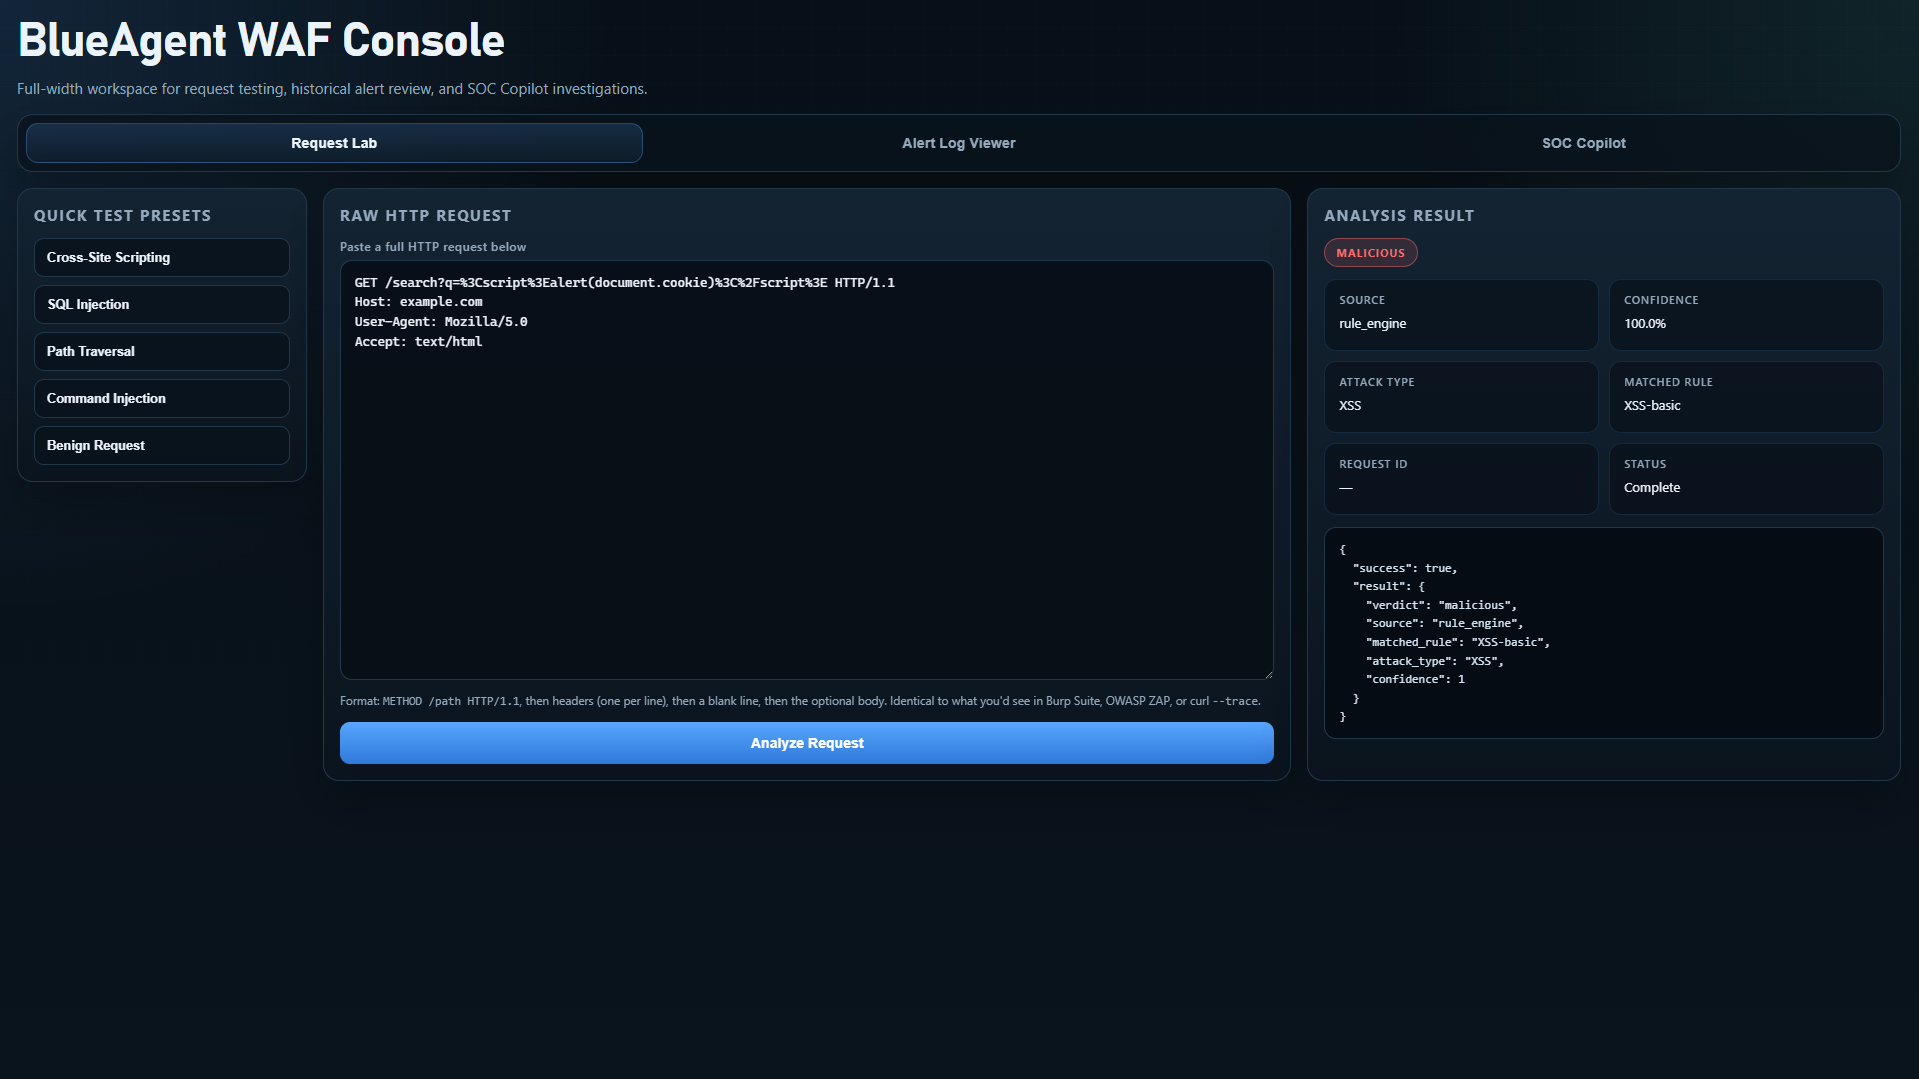
\includegraphics[width=0.92\textwidth]{images/pic/samplehttp.png}
    \caption{HTTP request sample in the BlueAgent WAF Console.}
    \label{fig:ai-console-sample-http}
\end{figure}

\subsubsection{AI Console Step 2: Sending an Analysis Prompt to the SOC Assistant}
After the request sample is available, the analyst can submit a targeted security question through the integrated SOC assistant prompt interface. This step validates that the system supports guided analyst interaction, allowing the operator to frame the investigation in a task-oriented way instead of relying only on fixed dashboard widgets. It also demonstrates that the AI layer is embedded in the same workflow used to inspect suspicious traffic.

\begin{figure}[H]
    \centering
    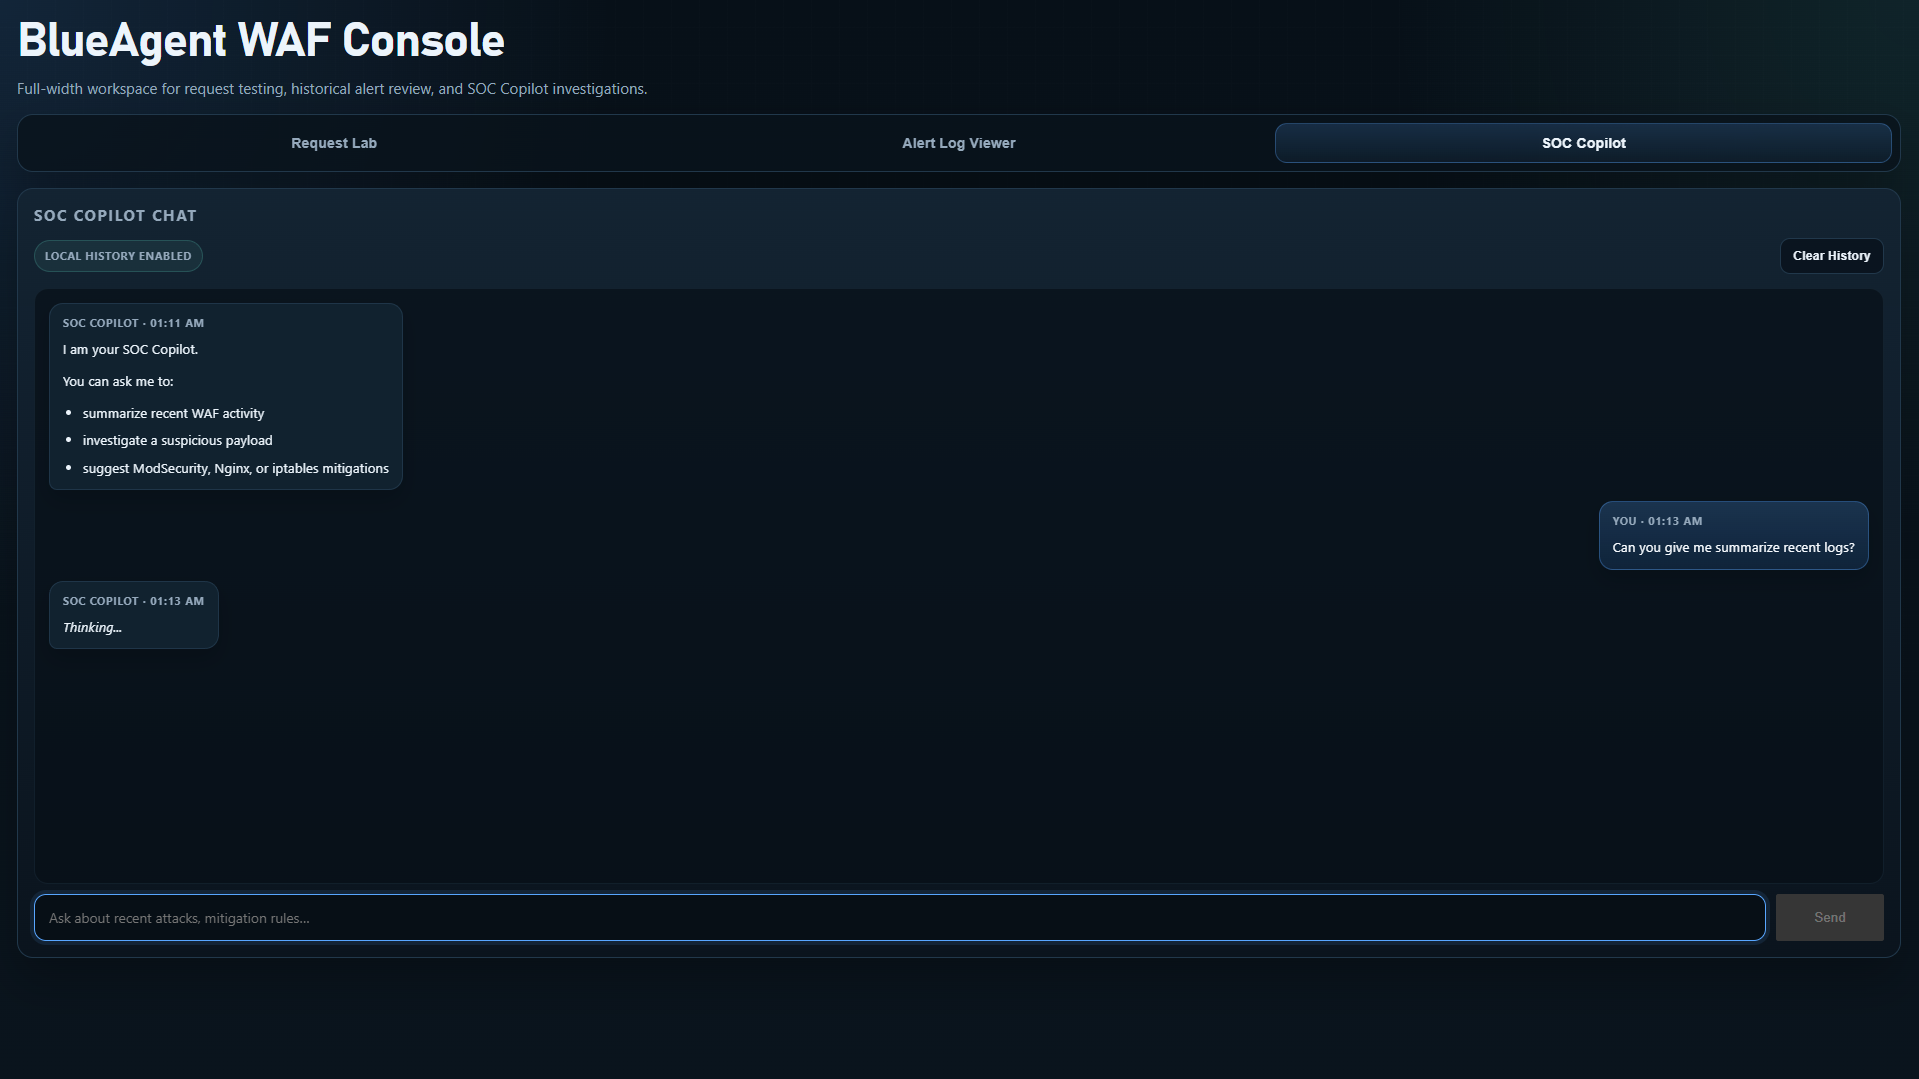
\includegraphics[width=0.92\textwidth]{images/pic/soc-ask.png}
    \caption{SOC assistant prompt in the BlueAgent WAF Console.}
    \label{fig:ai-console-soc-ask}
\end{figure}

\subsubsection{AI Console Step 3: Reviewing the Assistant's Security Interpretation}
The next validation step checks the generated AI response. The response panel shows that the SOC assistant can interpret the request content and return security-oriented observations that are usable during investigation. This matters because the aim of the feature is not only to call an LLM, but to obtain a concise explanation that helps the analyst understand why a request appears suspicious.

\begin{figure}[H]
    \centering
    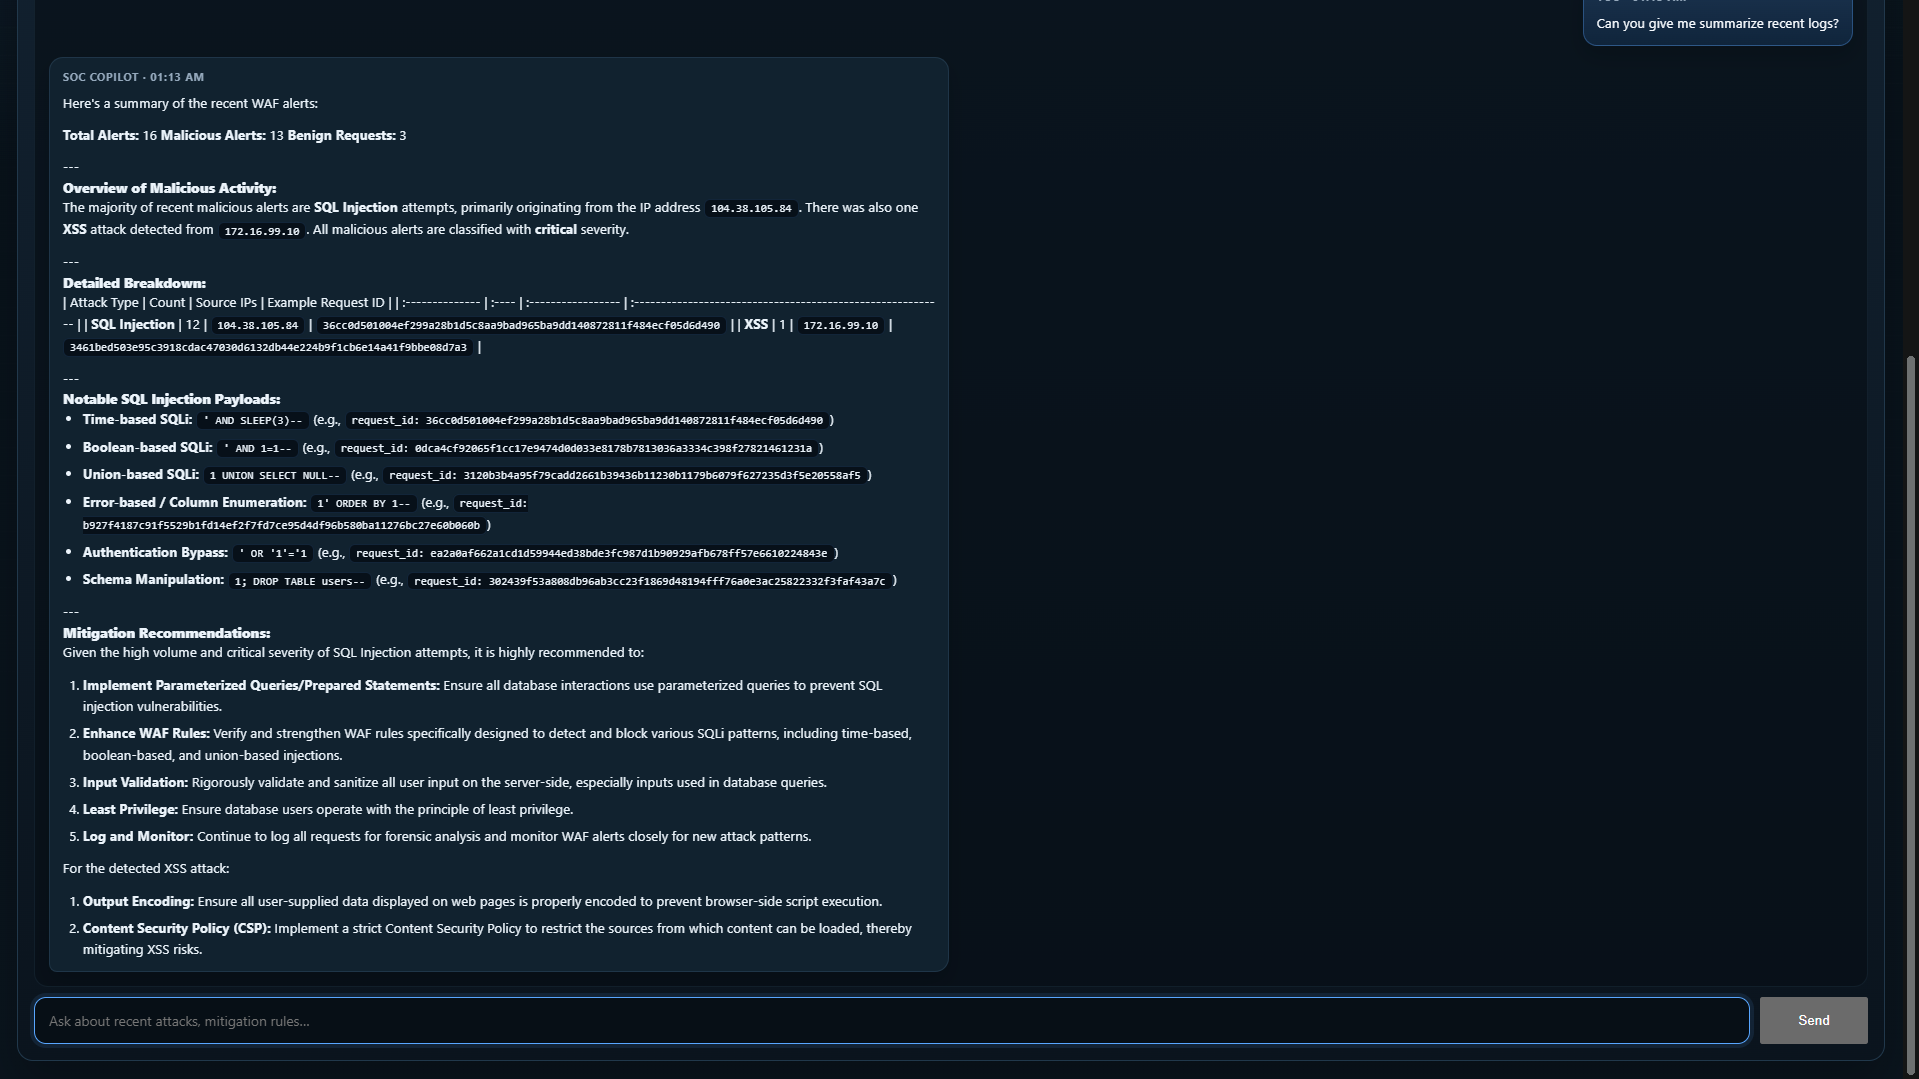
\includegraphics[width=0.92\textwidth]{images/pic/soc-answer.png}
    \caption{SOC assistant analysis output in the BlueAgent WAF Console.}
    \label{fig:ai-console-soc-answer}
\end{figure}

\subsubsection{AI Console Step 4: Using the SOC Copilot Investigation View}
The final console step validates the dedicated SOC copilot investigation view. This interface extends the earlier prompt-response interaction by presenting AI support in a more investigation-oriented layout, which is useful for analysts who need follow-up reasoning during alert review. From a validation perspective, this confirms that AI assistance is not limited to a single text response, but is integrated into a broader security-analysis workspace.

\begin{figure}[H]
    \centering
    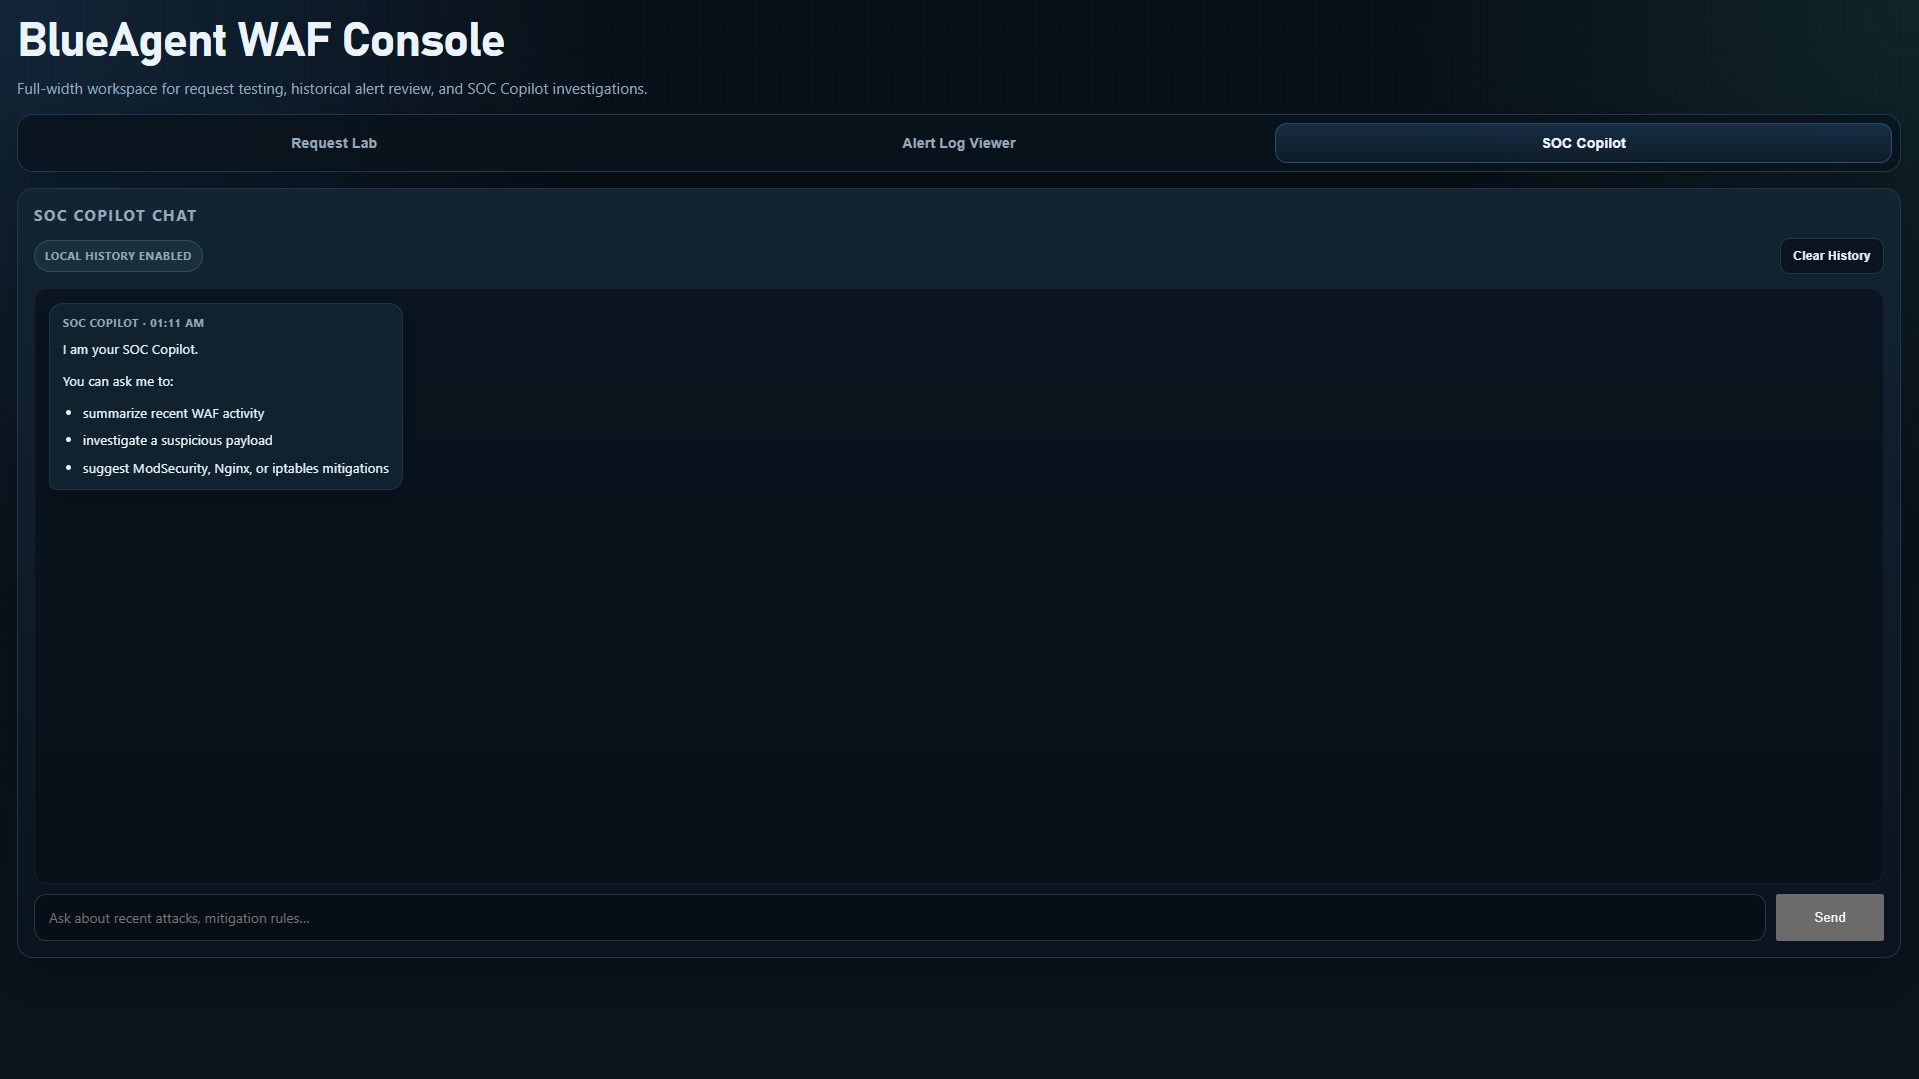
\includegraphics[width=0.92\textwidth]{images/pic/soc-coi.png}
    \caption{SOC copilot view in the BlueAgent WAF Console.}
    \label{fig:ai-console-soc-copilot}
\end{figure}




Taken together, these results validate that the platform supports both activation and practical use of AI-assisted analysis in a web-security training context.


\subsection{BlueTeam WAF Validation Workflow}
To make the BlueTeam capability assessment explicit, the project also validated a complete Web Application Firewall workflow using the BlueAgent WAF interface. In this workflow, each operational step was checked individually so that the report can show not only the final detection result, but also the configuration path that leads to that result. This is important in the capstone context because BlueTeam validation should demonstrate controllability, visibility, and investigation readiness rather than only a single alert outcome.

\subsubsection{Step 1: Accessing the BlueAgent WAF Interface}
The first step verifies that the operator can access the BlueAgent WAF through the login interface. This step confirms the availability of the defensive console and establishes the starting point of the BlueTeam workflow. From a validation perspective, successful access means that the analyst can reach the control surface used to review dashboards, inspect rules, and investigate later alerts.

\begin{figure}[H]
    \centering
    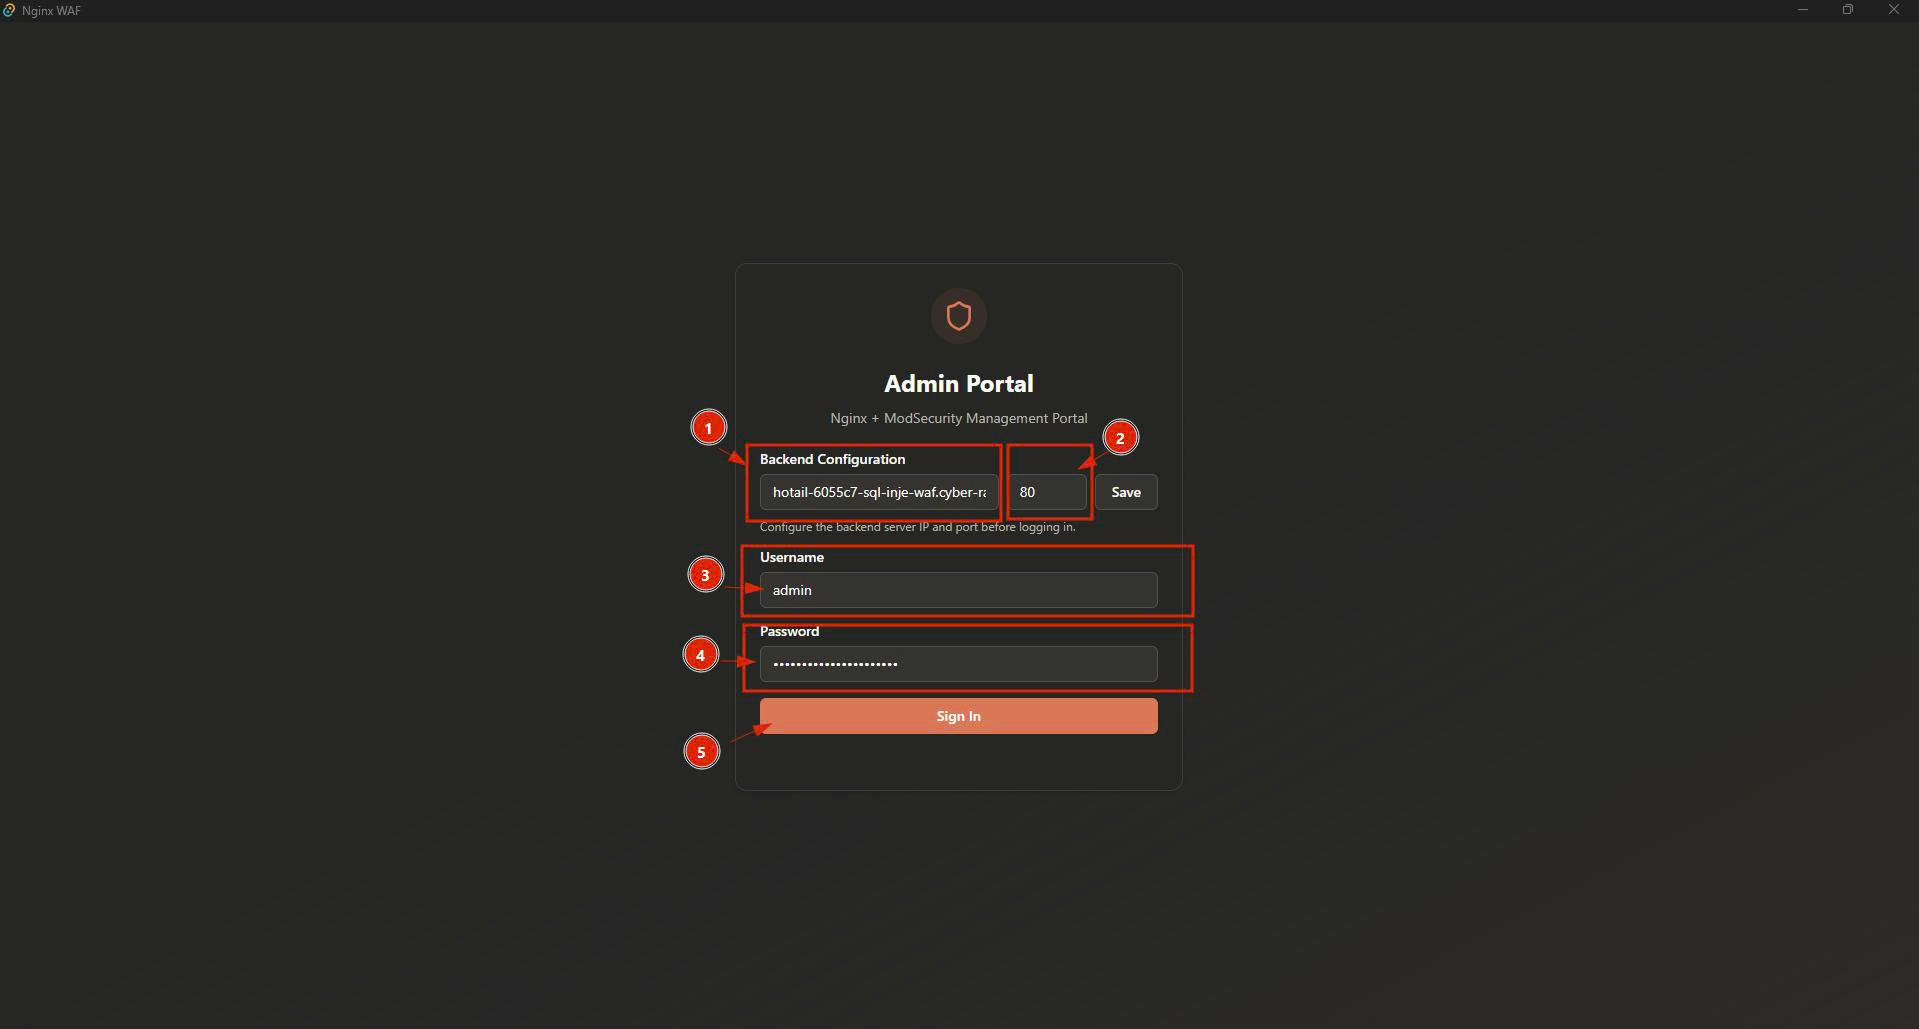
\includegraphics[width=0.82\textwidth]{images/pic/waf_login.jpg}
    \caption{BlueAgent WAF login interface.}
    \label{fig:blueteam-waf-login}
\end{figure}

\subsubsection{Step 2: Reviewing the Security Dashboard}
After successful login, the next step validates the dashboard view. The dashboard provides the BlueTeam operator with a consolidated overview of the protection system, allowing quick inspection of current security status before rule tuning or attack replay is performed. This step is useful because it shows that the platform supports operational awareness at the start of the defensive workflow rather than exposing only low-level logs.

\begin{figure}[H]
    \centering
    
\includegraphics[width=0.92\textwidth]{\detokenize{images/pic/waf dashboard.png}}
    \caption{BlueAgent WAF dashboard.}
    \label{fig:blueteam-waf-dashboard}
\end{figure}

\subsubsection{Step 3: Inspecting the SQL Injection Rule Before Activation}
The third step focuses on rule-management readiness. Before generating or replaying malicious traffic, the SQL Injection rule is inspected in its configuration interface to verify that the operator can review the relevant protection logic. This step demonstrates that the system exposes rule-level control to the BlueTeam user and that defensive behavior is not treated as a fixed black box.

\begin{figure}[H]
    \centering
    
\includegraphics[width=0.92\textwidth]{\detokenize{images/pic/rule sql.png}}
    \caption{SQL Injection rule before activation.}
    \label{fig:blueteam-sqli-rule-before}
\end{figure}

\subsubsection{Step 4: Confirming Successful SQL Injection Rule Activation}
After inspection, the SQL Injection rule is enabled and the system state is checked again. This step validates that defensive configuration changes can be applied successfully through the interface. In a BlueTeam workflow, this is a key checkpoint because the analyst must be able to move from passive observation to active protection policy enforcement.

\begin{figure}[H]
    \centering
    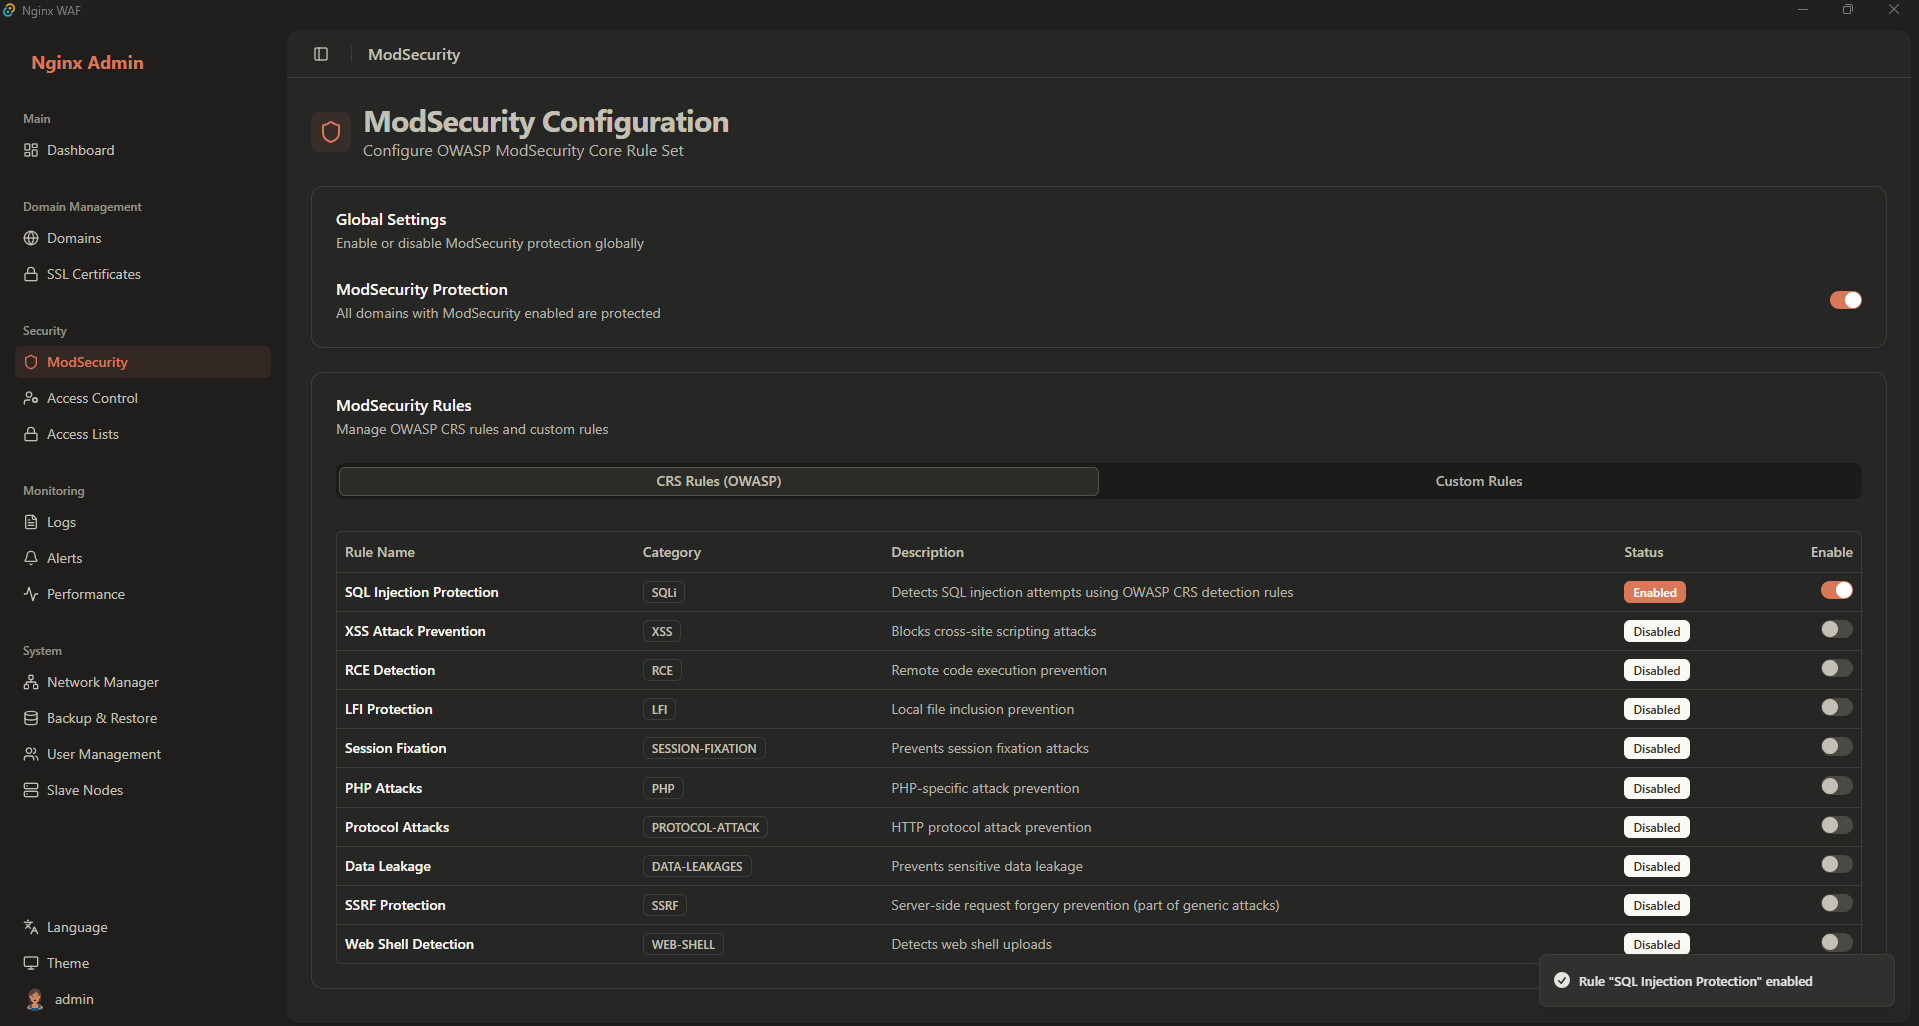
\includegraphics[width=0.92\textwidth]{images/pic/rulesqlsuccess.png}
    \caption{SQL Injection rule after activation.}
    \label{fig:blueteam-sqli-rule-after}
\end{figure}

\subsubsection{Step 5: Reviewing Security Logs After Rule Enforcement}
Once the rule is active, the validation continues by reviewing the generated security logs. This step confirms that suspicious requests are not only blocked or classified internally, but are also recorded in a way that supports later review. The captured evidence shows that the platform can present malicious web activity such as SQL Injection and XSS within the BlueTeam monitoring flow, which is essential for both training and incident analysis.

\begin{figure}[H]
    \centering
    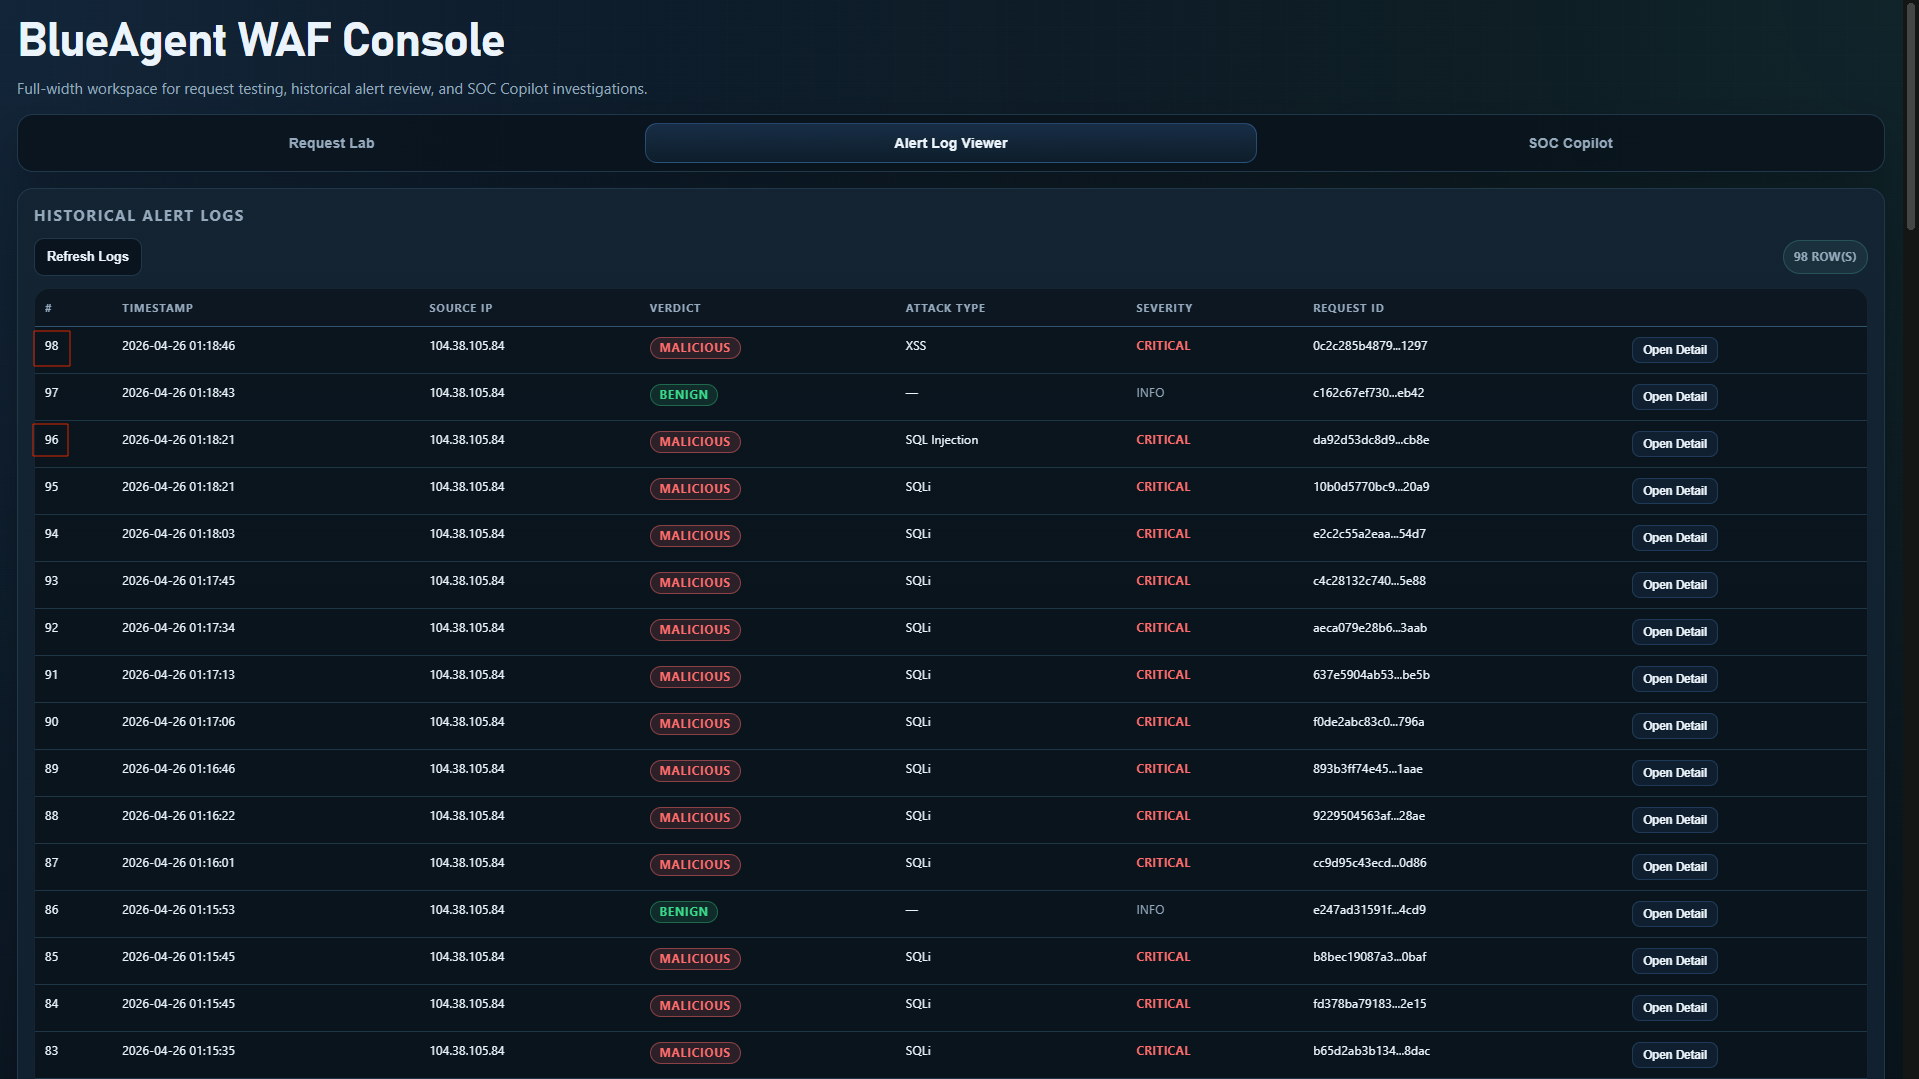
\includegraphics[width=0.92\textwidth]{images/pic/logs-rule.png}
    \caption{Security logs after rule enforcement.}
    \label{fig:blueteam-logs-rule}
\end{figure}

\subsubsection{Step 6: Investigating the Alert in Detail}
The final step validates analyst investigation capability. After a suspicious request is detected, the alert-detail view is opened to inspect the verdict, severity, attack type, source IP, HTTP method, and event payload. This is the most important evidence in the BlueTeam chain because it shows that the system does not stop at coarse alert generation; it also preserves enough context for technical interpretation and post-event analysis. The detailed JSON record strengthens the validation by proving that the platform retains structured evidence for security review.

\begin{figure}[H]
    \centering
    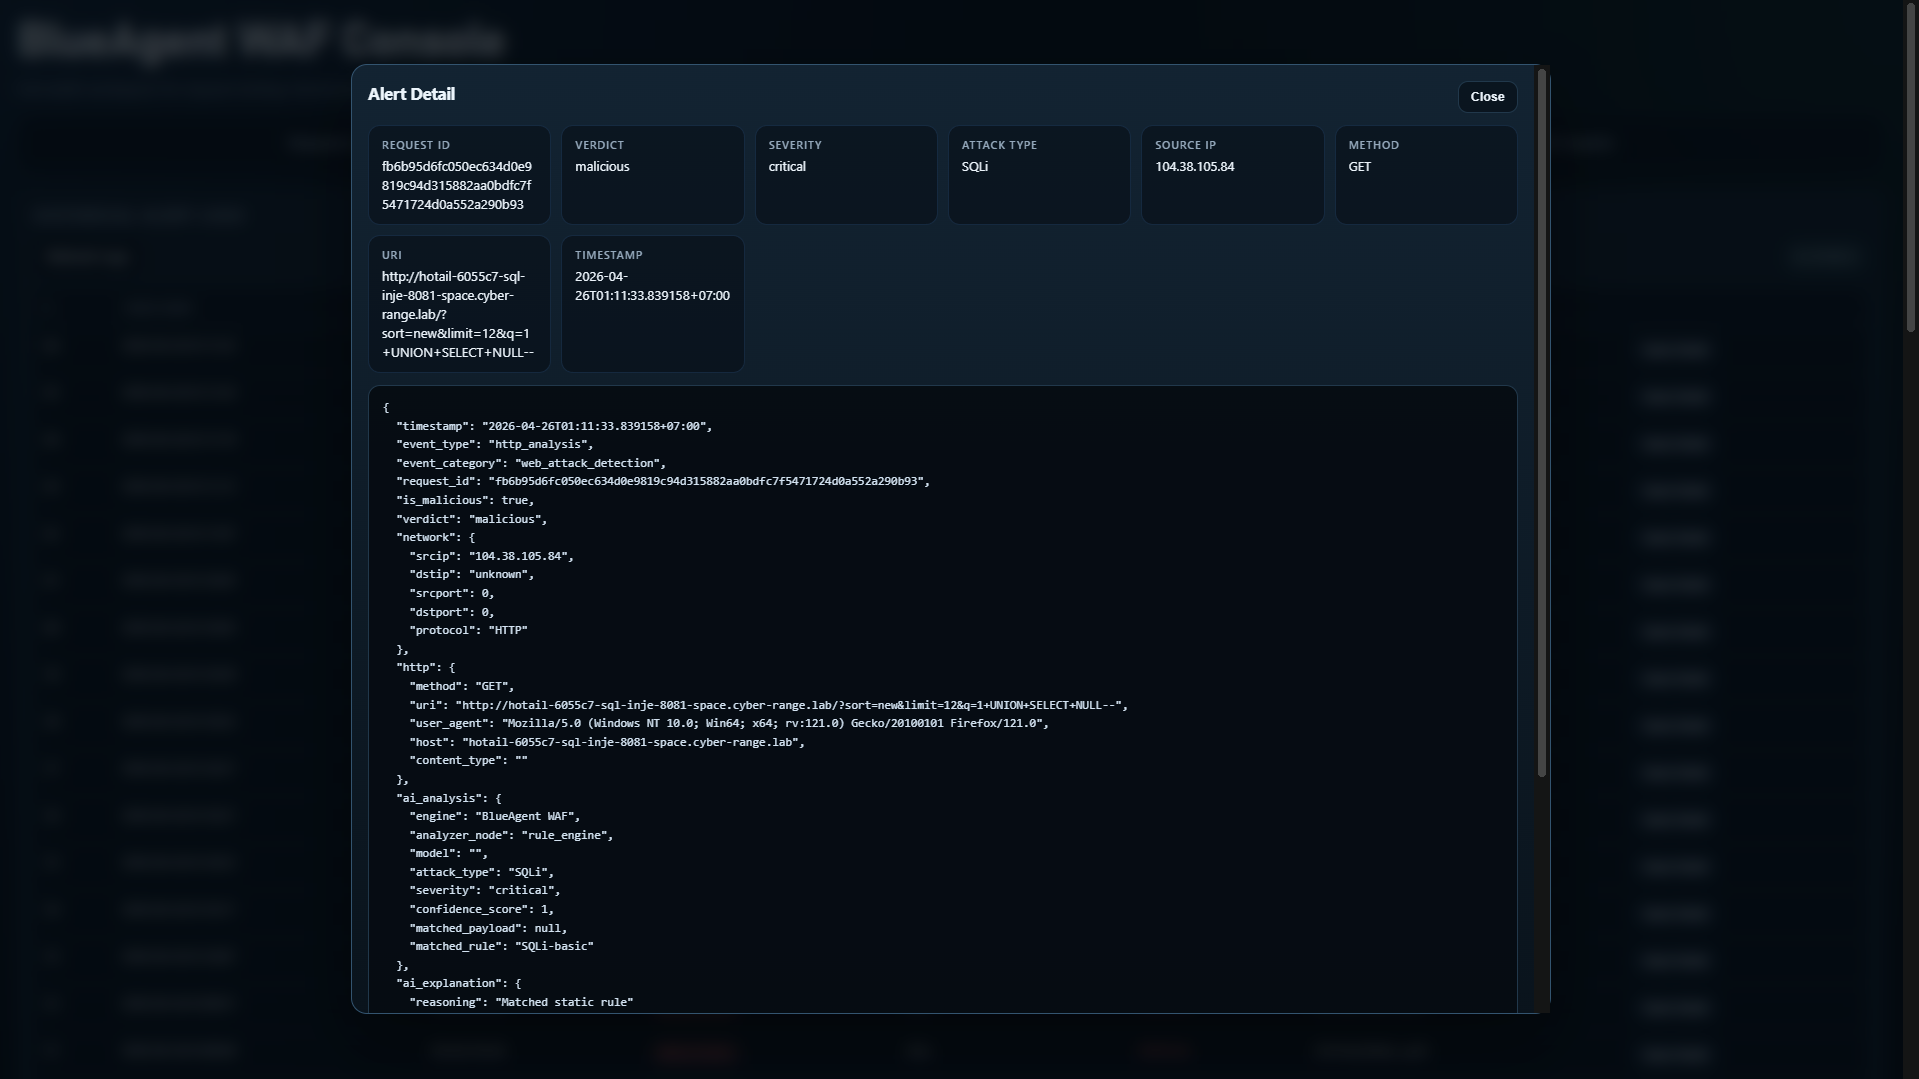
\includegraphics[width=0.92\textwidth]{images/pic/alert-detail.png}
    \caption{Detailed SQL Injection alert in BlueAgent WAF.}
    \label{fig:blueteam-alert-detail}
\end{figure}

Taken together, these six steps validate a complete BlueTeam workflow: the operator can access the defensive console, review the security dashboard, inspect and activate a protection rule, observe the resulting security logs, and investigate the generated alert in detail. Presenting each screenshot separately is important because it demonstrates operational continuity across the full defensive process rather than compressing multiple validation checkpoints into a single composite image.


\subsection{RedTeam AI-Assisted Attack Workflow}
The Red Team capability was also validated through a guided attack workflow built around the Cyber Shell Assistant and the vulnerable SQL App target. Unlike the BlueTeam workflow, which emphasizes monitoring and investigation, this Red Team workflow focuses on target discovery, session-aware assistant interaction, command guidance, and command execution against the web target. The provided PDF and screenshot sequence show that the assistant is not acting as an autonomous attacker; instead, it supports the learner by observing shell context, identifying the target, and suggesting commands that the user executes in the terminal.

\subsubsection{Step 1: Accessing the Cyber Shell Assistant}
The first step validates that the learner can access the Cyber Shell Assistant interface. This interface provides the session list, the captured shell-event history, and the chat panel used for AI-guided interaction. It serves as the main Red Team workspace for combining terminal activity with assistant feedback.

\begin{figure}[H]
    \centering
    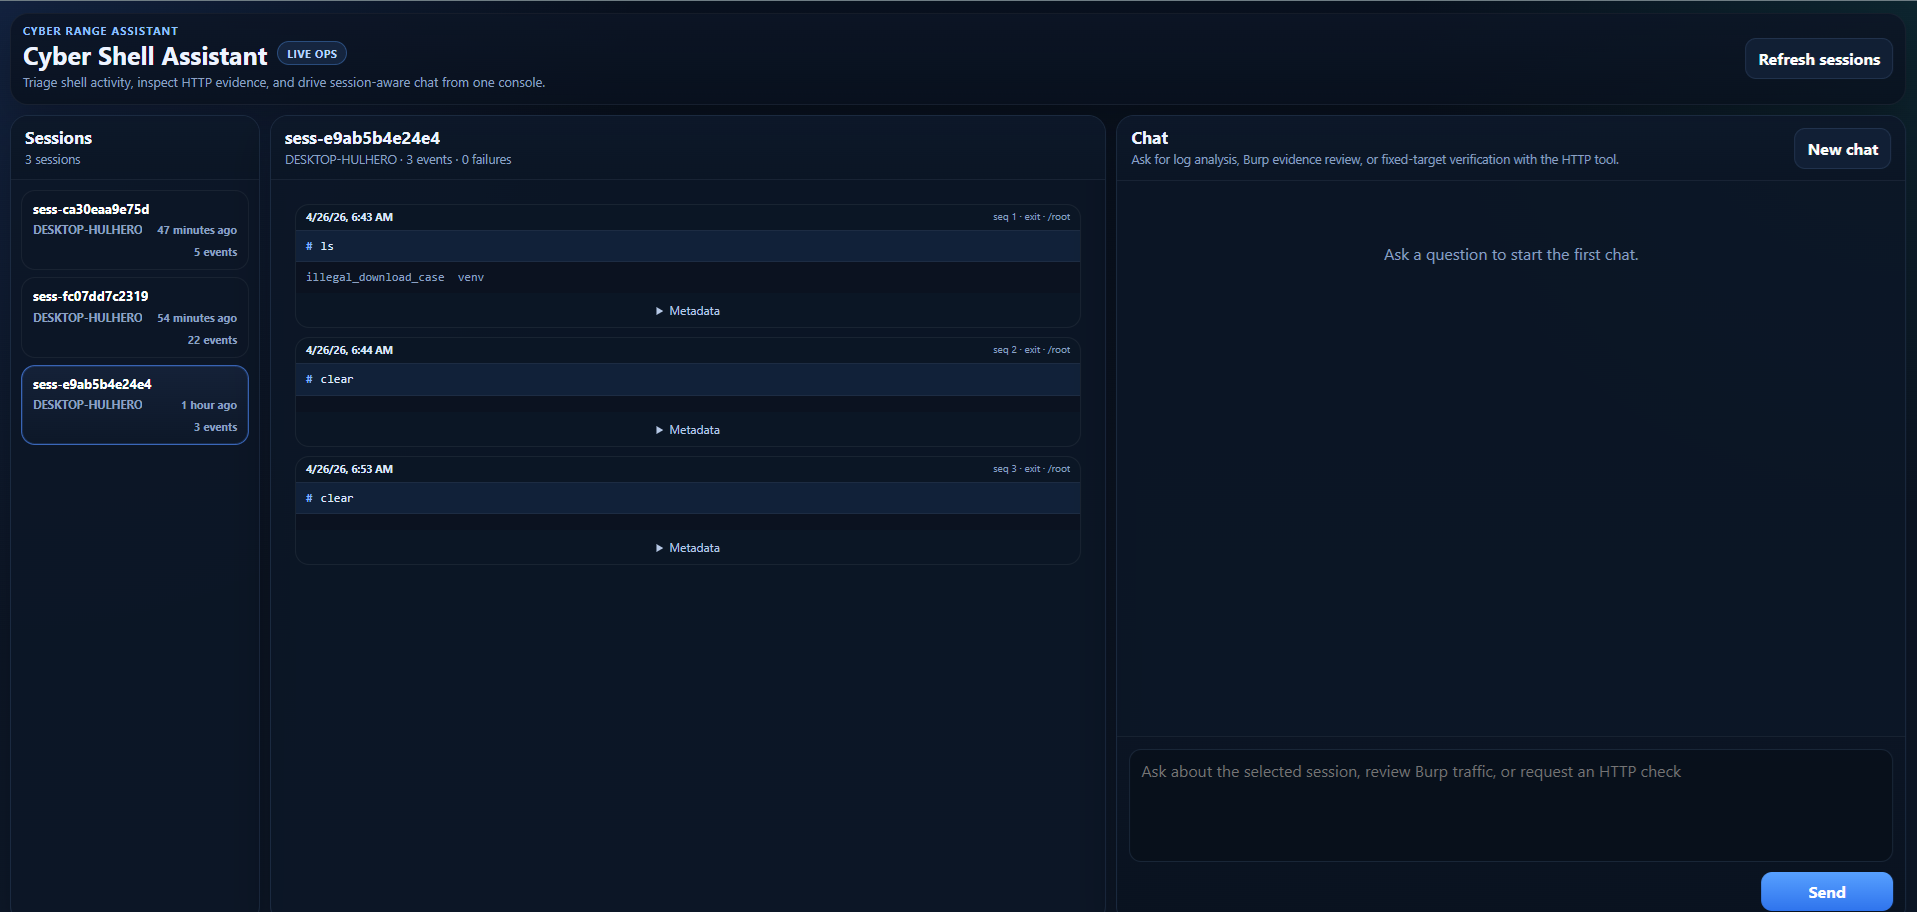
\includegraphics[width=0.92\textwidth]{images/cyred/cyred/1.png}
    \caption{Cyber Shell Assistant interface.}
    \label{fig:redteam-cybershell-interface}
\end{figure}

\subsubsection{Step 2: Opening the Target Web Application}
The second step confirms the availability of the target application used in the exercise. In this case, the learner is given access to the SQL App web target, which exposes searchable product data and becomes the focus of later SQL injection testing. This step establishes the attack surface before the learner interacts with the assistant.

\begin{figure}[H]
    \centering
    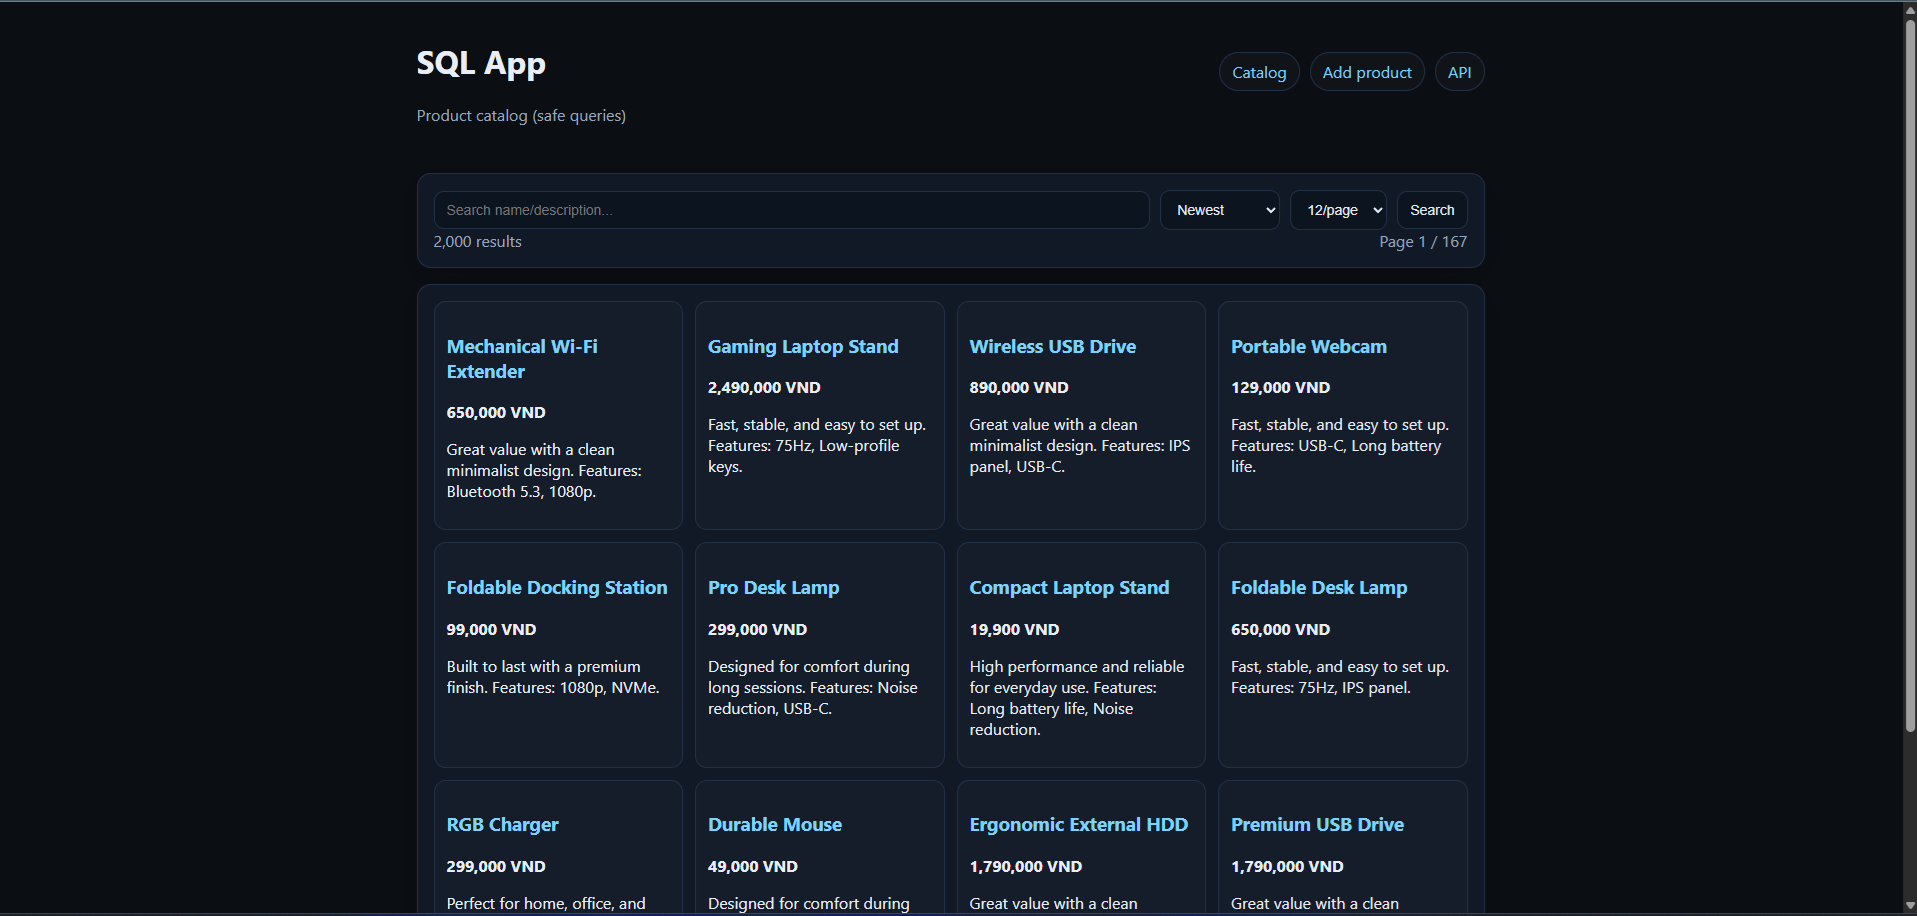
\includegraphics[width=0.92\textwidth]{images/cyred/cyred/2.png}
    \caption{SQL App target interface.}
    \label{fig:redteam-sqlapp-target}
\end{figure}

\subsubsection{Step 3: Connecting the Terminal to the Cyber Shell Assistant}
Before the assistant can reason over shell activity, the learner must connect the local terminal to the Cyber Shell service using the provided command. This step validates the telemetry bridge between terminal actions and the web dashboard. Once this connection is established, shell commands become visible in the assistant session and can later be used as context for AI responses.

\begin{figure}[H]
    \centering
    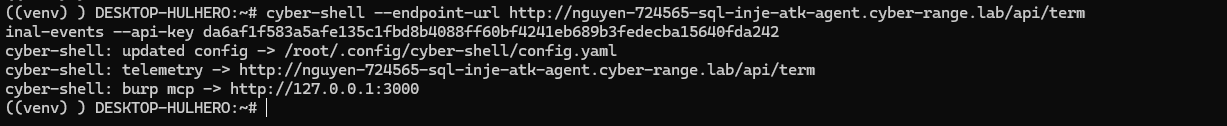
\includegraphics[width=0.92\textwidth]{images/cyred/cyred/3.png}
    \caption{Terminal connection to Cyber Shell.}
    \label{fig:redteam-terminal-connect}
\end{figure}

\subsubsection{Step 4: Verifying Session Synchronization on the Dashboard}
After terminal setup, the dashboard is checked to confirm that the new shell session and its recent commands are visible in the Cyber Shell Assistant interface. This validation step is important because the later AI guidance depends on accurate session awareness. The synchronized session history shows that the assistant can ground its responses in actual learner activity instead of relying only on manually typed prompts.

\begin{figure}[H]
    \centering
    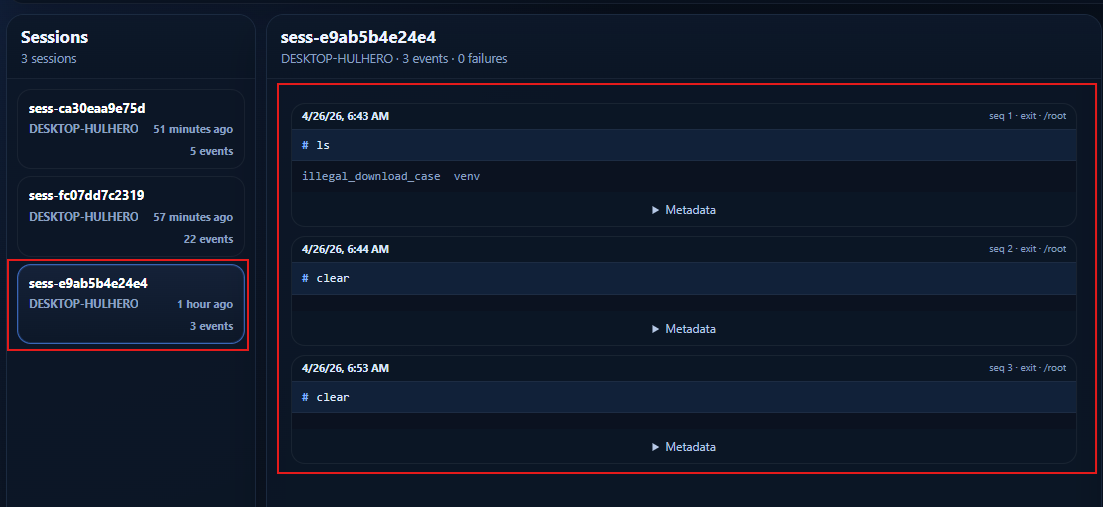
\includegraphics[width=0.92\textwidth]{images/cyred/cyred/4.png}
    \caption{Synchronized shell session in the dashboard.}
    \label{fig:redteam-session-sync}
\end{figure}

\subsubsection{Step 5: Probing the Target from the Terminal}
Once the session is active, the learner issues a direct \texttt{curl} request to the SQL App target. This step allows the assistant to observe which web target is being explored and also confirms that the target is reachable from the attack environment. The returned HTML output exposes the application structure and provides context for later exploitation steps.

\begin{figure}[H]
    \centering
    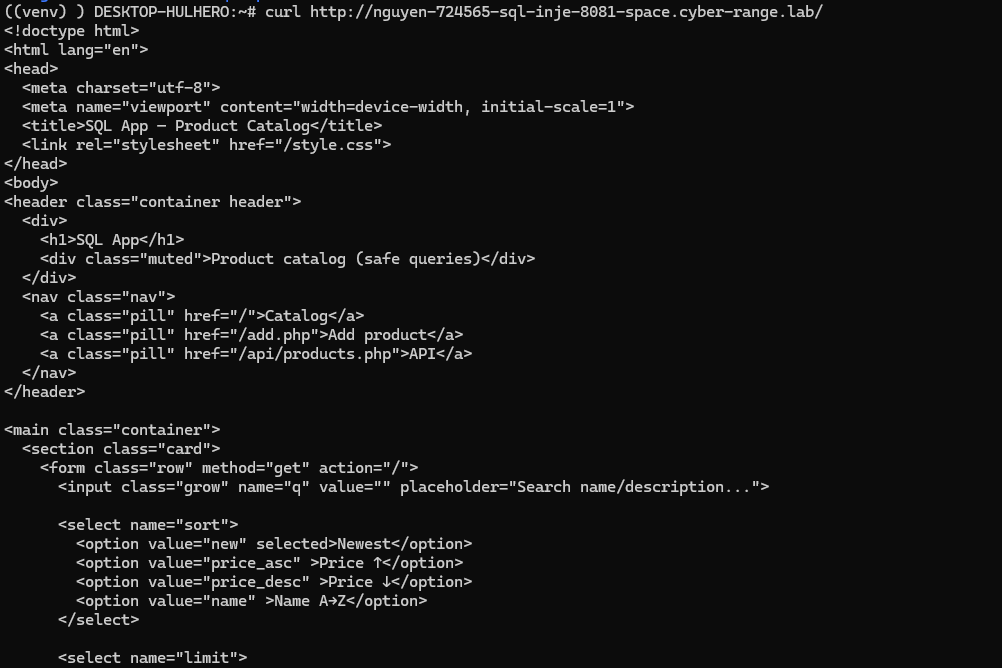
\includegraphics[width=0.92\textwidth]{images/cyred/cyred/5.png}
    \caption{Initial \texttt{curl} request to the target.}
    \label{fig:redteam-curl-target}
\end{figure}

\subsubsection{Step 6: Asking the Assistant to Identify the Target}
After the target is probed, the learner asks the Cyber Shell Assistant whether it can detect the website being targeted. The assistant answers using the recent shell history and demonstrates tool-assisted awareness by identifying the SQL App target and confirming that it can reach the application with an HTTP request. This step validates that the Red Team copilot is context-aware and can reason from captured terminal evidence.

\begin{figure}[H]
    \centering
    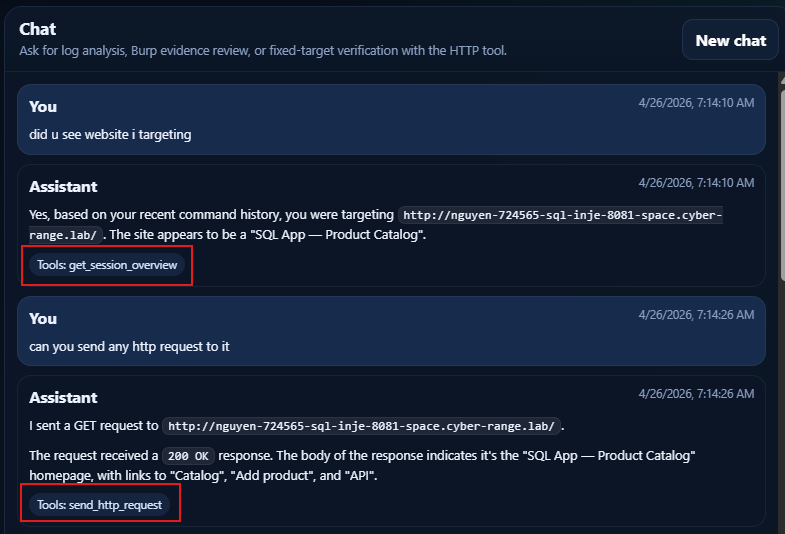
\includegraphics[width=0.92\textwidth]{images/cyred/cyred/6.png}
    \caption{Assistant identifies the target website.}
    \label{fig:redteam-assistant-identify-target}
\end{figure}

\subsubsection{Step 7: Requesting SQL Injection Guidance}
The next step validates AI-assisted offensive guidance. The learner asks how to check for SQL injection in the \texttt{q} URL parameter and how to use \texttt{sqlmap} to enumerate databases. The assistant responds with a command template that the learner can execute manually. This confirms that the assistant supports the learning process by suggesting relevant attack commands without directly carrying out the attack on its own.

\begin{figure}[H]
    \centering
    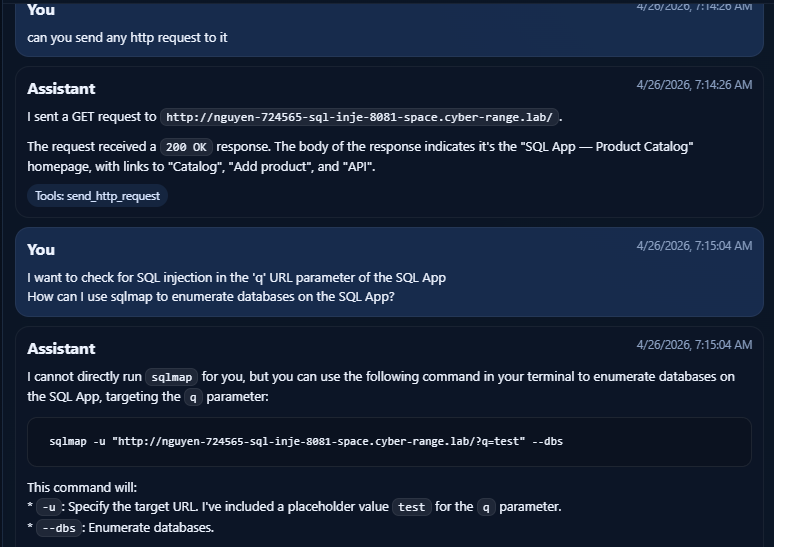
\includegraphics[width=0.92\textwidth]{images/cyred/cyred/7.png}
    \caption{Assistant guidance for SQL injection testing.}
    \label{fig:redteam-assistant-sqli-guidance}
\end{figure}

\subsubsection{Step 8: Enumerating Databases with \texttt{sqlmap}}
Following the assistant's suggestion, the learner executes the enumeration command in the terminal. The result shows that the backend DBMS is MySQL-compatible and that available databases include \texttt{information\_schema} and \texttt{shop\_db}. This step provides concrete exploitation evidence and validates that the guided command leads to a meaningful offensive result.

\begin{figure}[H]
    \centering
    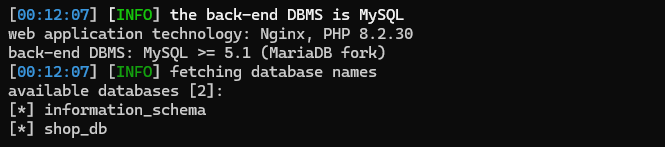
\includegraphics[width=0.92\textwidth]{images/cyred/cyred/8.png}
    \caption{Database enumeration with \texttt{sqlmap}.}
    \label{fig:redteam-sqlmap-dbs}
\end{figure}

\subsubsection{Step 9: Requesting Data-Dump Guidance}
After confirming the presence of the target database, the learner asks the assistant for a command to dump the data. The assistant returns a \texttt{sqlmap} command that targets \texttt{shop\_db} and uses the dump option. This step extends the earlier guidance from reconnaissance and enumeration toward data extraction and shows that the assistant can support multi-step offensive workflows.

\begin{figure}[H]
    \centering
    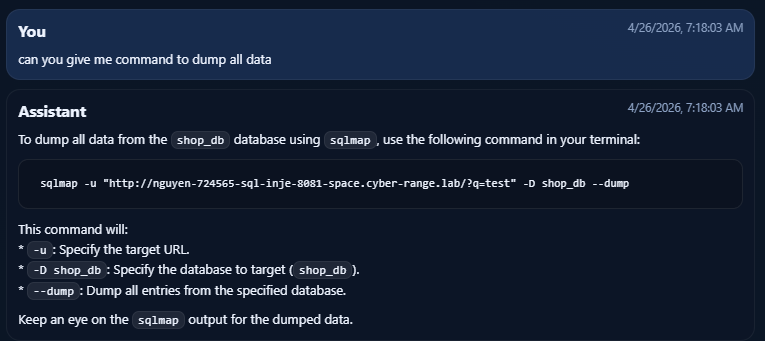
\includegraphics[width=0.92\textwidth]{images/cyred/cyred/9.png}
    \caption{Assistant guidance for dumping database content.}
    \label{fig:redteam-assistant-dump-guidance}
\end{figure}

\subsubsection{Step 10: Dumping Table Data from the Target Database}
In the final step, the learner executes the dump command and obtains table data from the \texttt{shop\_db} database. The terminal output shows fetched tables, columns, and product entries, demonstrating that the attack workflow progressed from target identification to database enumeration and then to data extraction. This final result validates the Red Team learning flow as an AI-assisted, session-aware attack exercise grounded in actual terminal interaction.

\begin{figure}[H]
    \centering
    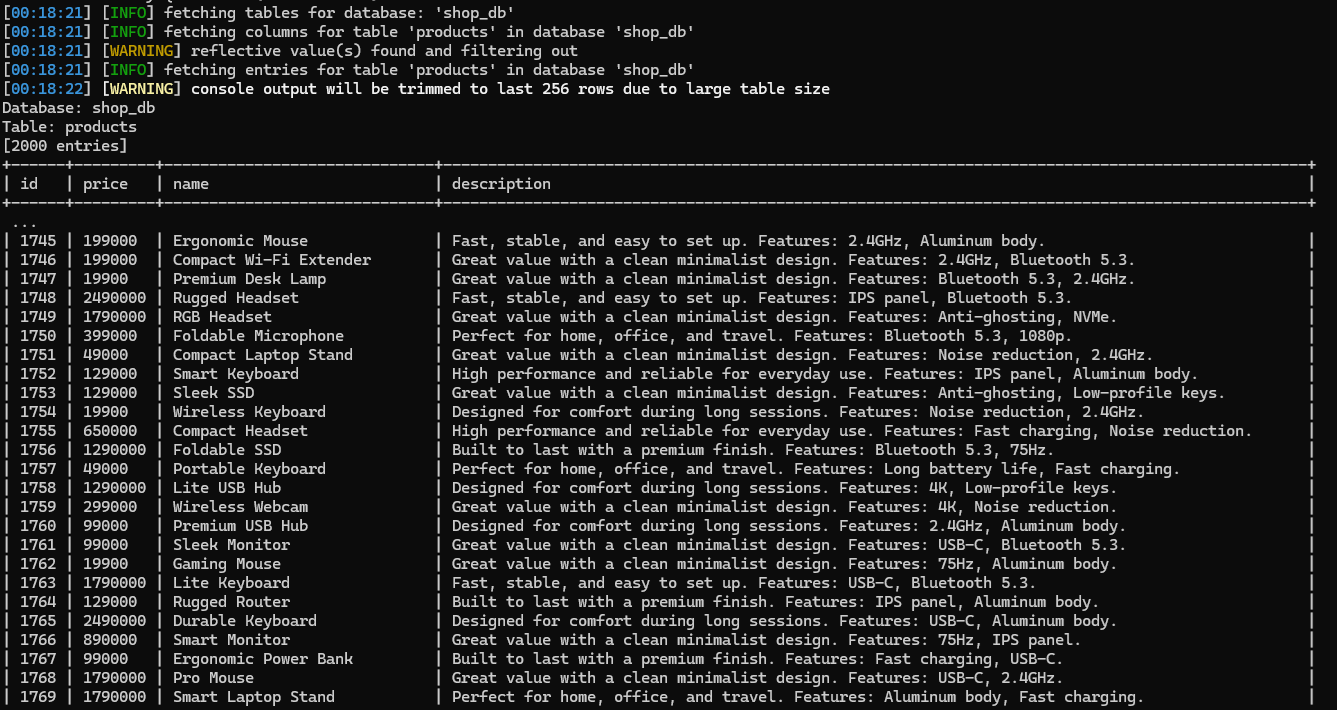
\includegraphics[width=0.92\textwidth]{images/cyred/cyred/10.png}
    \caption{Dumped data from \texttt{shop\_db}.}
    \label{fig:redteam-sqlmap-dump}
\end{figure}

Taken together, these ten steps validate a complete Red Team workflow: the learner accesses the Cyber Shell Assistant, connects the terminal, confirms session synchronization, probes the target, receives AI guidance, and executes offensive commands that enumerate and dump database content from the vulnerable web application. This evidence is especially valuable because it shows that the AI component supports hands-on offensive learning through contextual guidance rather than by replacing user action.


\subsection{RAG and No-RAG Benchmark Comparison}
A controlled benchmark was conducted to compare RAG and No-RAG on the same 800-request dataset. The comparison focuses on detection, attack intelligence, and grounded reasoning.

The results show that RAG is most valuable for semantic interpretation and grounded reasoning.

\subsubsection{Core Detection Performance}
Table~\ref{tab:core-detection-rag-vs-norag} summarizes the main detection metrics.

\begin{table}[H]
    \centering
    \small
    \setlength{\tabcolsep}{5pt}
    \renewcommand{\arraystretch}{1.15}
    \begin{tabularx}{\textwidth}{|X|c|c|c|}
        \hline
        \textbf{Metric} & \textbf{RAG} & \textbf{No-RAG} & \textbf{Observation} \\
        \hline
        Accuracy & 88.38\% & 88.38\% & Equivalent overall classification accuracy \\
        \hline
        Precision & 95.10\% & 93.80\% & RAG reduces false malicious predictions \\
        \hline
        F1-score & 93.23\% & 93.32\% & Comparable overall detection balance \\
        \hline
        Specificity & 67.00\% & 57.00\% & RAG better distinguishes benign traffic \\
        \hline
        False positive rate & 33.00\% & 43.00\% & RAG lowers benign misclassification \\
        \hline
    \end{tabularx}
    \caption{Core detection comparison.}
    \label{tab:core-detection-rag-vs-norag}
\end{table}

RAG keeps overall detection stable while improving precision and specificity.

The same tendency is visible in the overall comparison chart, where accuracy remains unchanged while precision and groundedness improve under the RAG setting.

\begin{figure}[H]
    \centering
    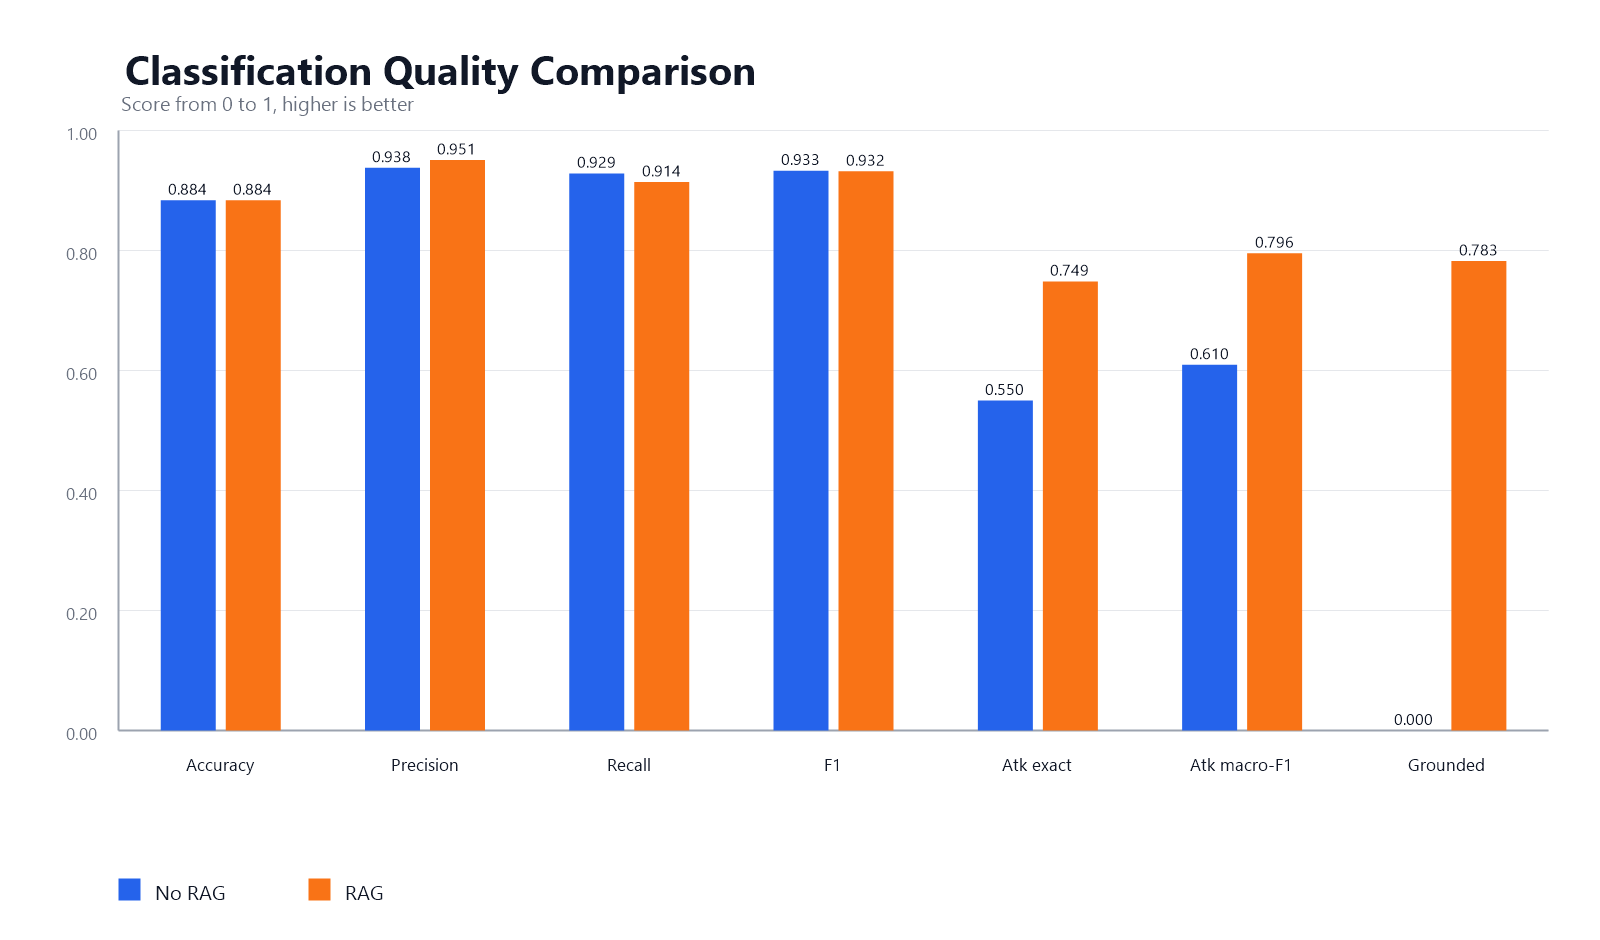
\includegraphics[width=0.95\textwidth]{images/chart_overall_comparison.png}
    \caption{Overall classification quality comparison.}
    \label{fig:rag-overall-comparison}
\end{figure}

\subsubsection{Attack-Intelligence Comparison}
The benchmark also measures how accurately the system identifies the attack family.

\begin{table}[H]
    \centering
    \small
    \setlength{\tabcolsep}{5pt}
    \renewcommand{\arraystretch}{1.15}
    \begin{tabularx}{\textwidth}{|X|c|c|c|}
        \hline
        \textbf{Metric} & \textbf{RAG} & \textbf{No-RAG} & \textbf{Observation} \\
        \hline
        Joint exact match accuracy & 74.86\% & 55.00\% & RAG strongly improves exact verdict+type correctness \\
        \hline
        Conditional exact match accuracy & 81.88\% & 59.23\% & RAG yields more accurate attack-family assignment \\
        \hline
        Macro-F1 for attack type & 79.55\% & 60.97\% & RAG improves balanced multi-class attack recognition \\
        \hline
    \end{tabularx}
    \caption{Attack-intelligence comparison.}
    \label{tab:attack-intelligence-rag-vs-norag}
\end{table}

RAG produces a clear improvement in attack-type intelligence.

This improvement is easier to observe in the per-attack visualization, where most attack families achieve a higher F1-score with RAG, especially SSI, LDAP Injection, SQL Injection, and XPath Injection.

\begin{figure}[H]
    \centering
    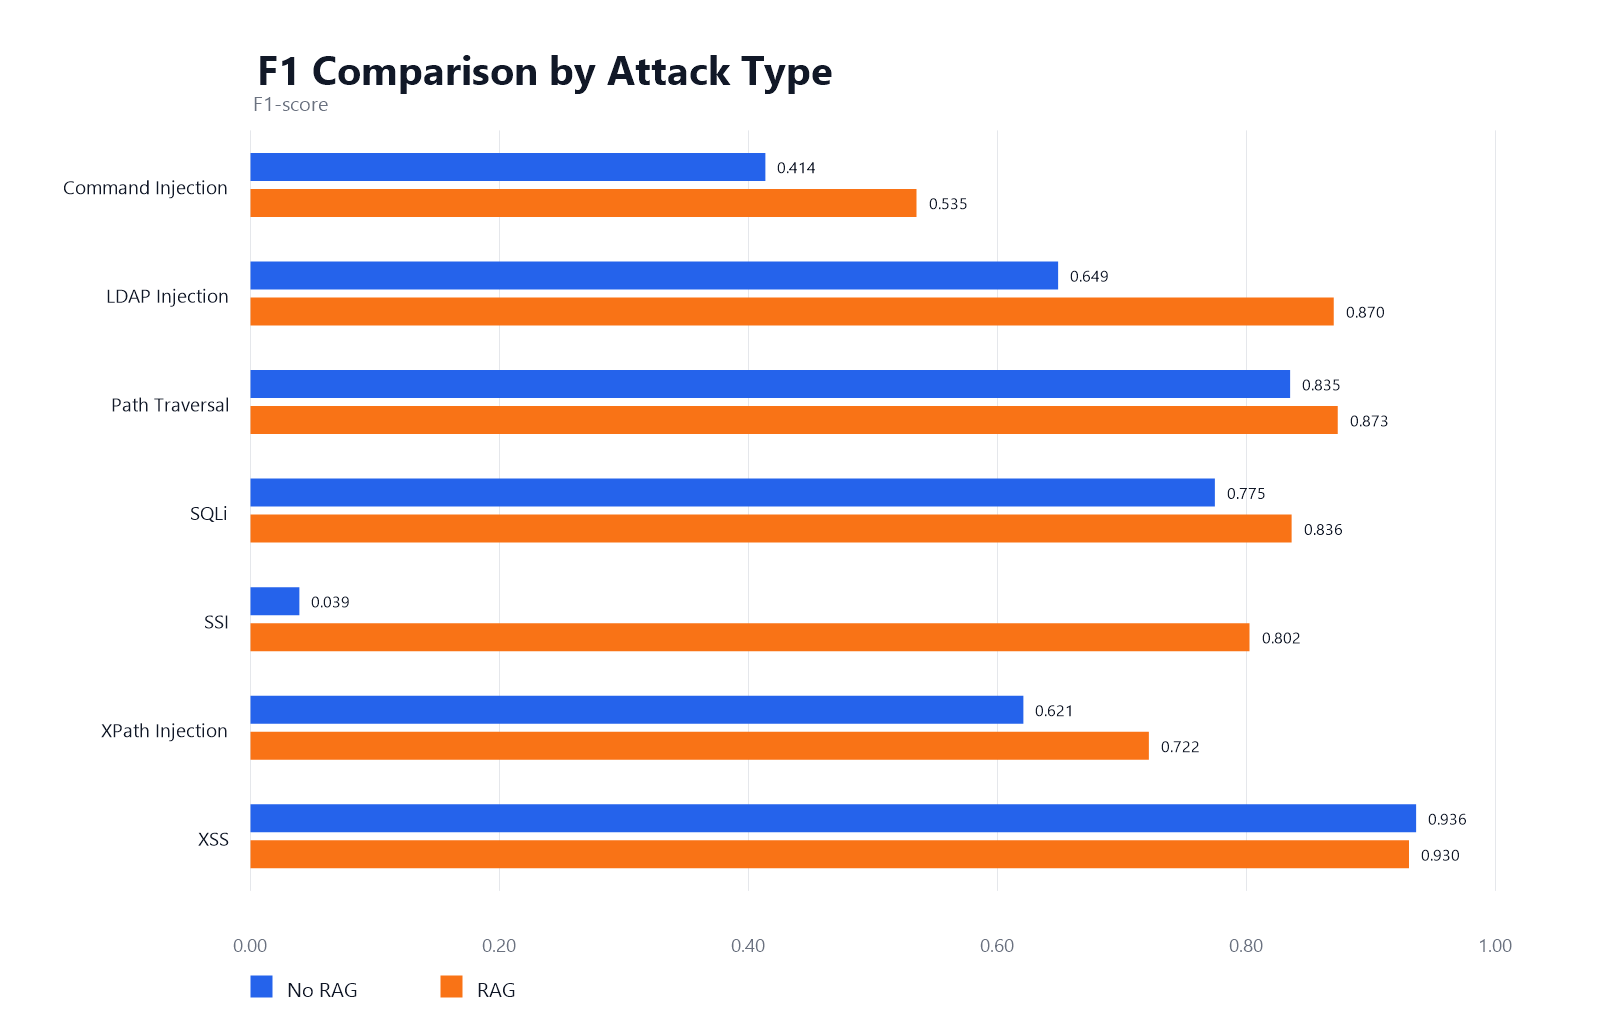
\includegraphics[width=0.95\textwidth]{images/chart_attack_type_f1_comparison.png}
    \caption{F1-score comparison by attack type.}
    \label{fig:rag-attack-type-f1}
\end{figure}

\subsubsection{Reasoning and Groundedness Comparison}
The final comparison evaluates whether LLM outputs remain evidence-grounded.

\begin{table}[H]
    \centering
    \small
    \setlength{\tabcolsep}{5pt}
    \renewcommand{\arraystretch}{1.15}
    \begin{tabularx}{\textwidth}{|X|c|c|c|}
        \hline
        \textbf{Metric} & \textbf{RAG} & \textbf{No-RAG} & \textbf{Observation} \\
        \hline
        LLM-path label accuracy & 91.79\% & 88.64\% & RAG improves verdict quality on LLM-routed samples \\
        \hline
        LLM-path attack-type accuracy & 89.86\% & 52.95\% & RAG greatly improves semantic interpretation \\
        \hline
        True attack type in top-k retrieval & 82.61\% & 0.00\% & Only RAG provides relevant retrieved support \\
        \hline
        Predicted attack type in top-k retrieval & 78.99\% & 0.00\% & RAG aligns generated output with retrieved context \\
        \hline
        Grounded correct rate & 78.26\% & 0.00\% & Grounded reasoning is only present with RAG \\
        \hline
        Eligible malicious LLM samples & 414 & 440 & Similar LLM-evaluated malicious volume \\
        \hline
    \end{tabularx}
    \caption{Reasoning and groundedness comparison.}
    \label{tab:groundedness-rag-vs-norag}
\end{table}

Overall, RAG mainly improves explanation quality, semantic accuracy, and groundedness.

\subsubsection{Latency Comparison}
The benchmark also considered the latency cost introduced by retrieval. As expected, the RAG pipeline is slower because it adds embedding, vector retrieval, and prompt augmentation before generation. However, the added latency remains acceptable for an academic cyber-range setting where explanation quality and grounded reasoning are more important than ultra-low response time.

\begin{figure}[H]
    \centering
    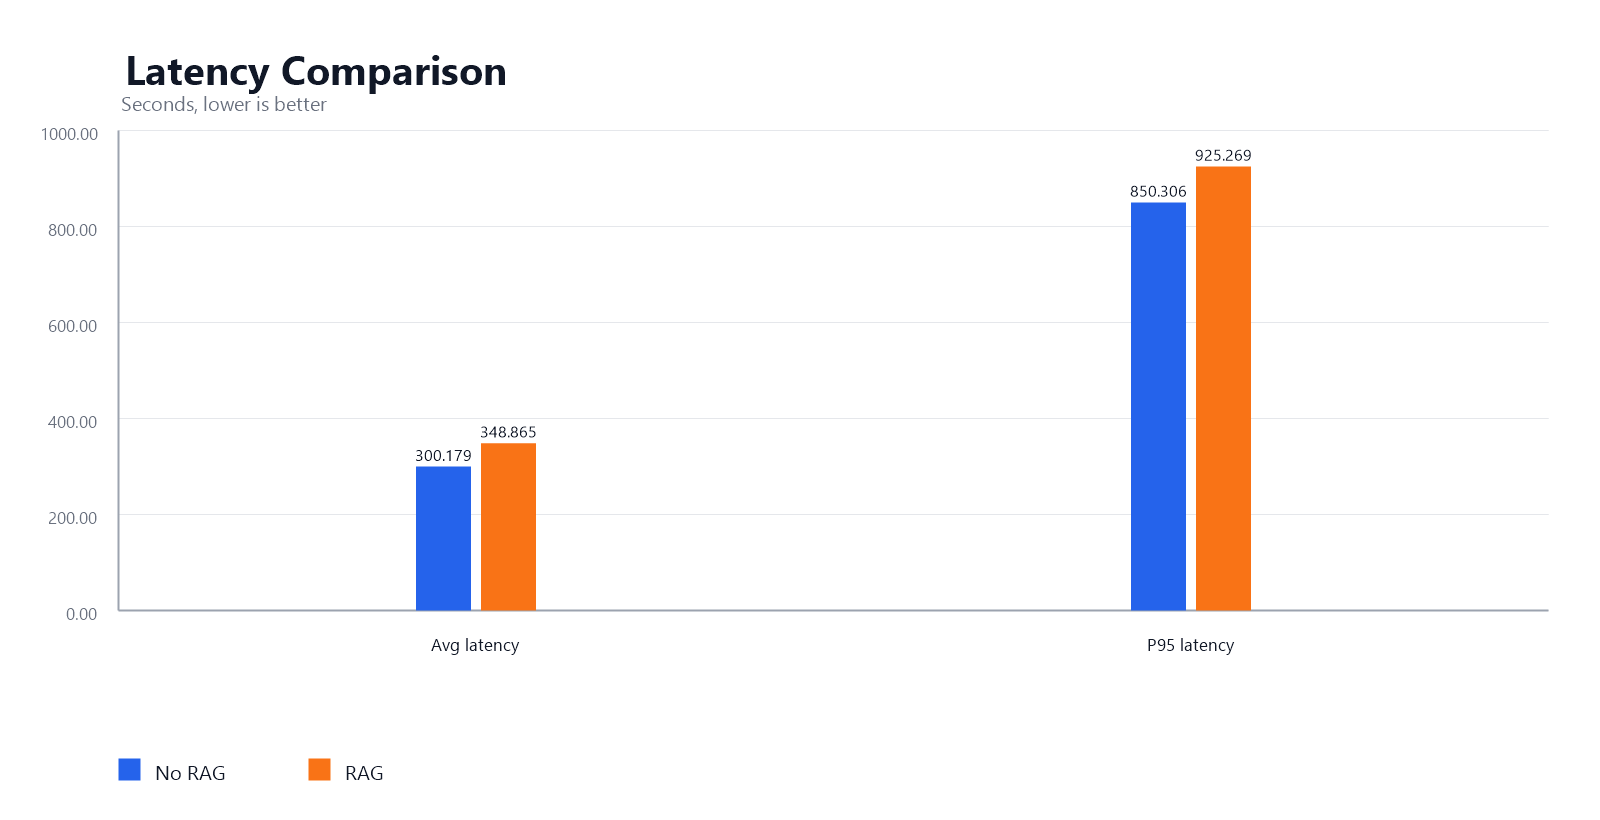
\includegraphics[width=0.95\textwidth]{images/chart_latency_comparison.png}
    \caption{Latency comparison between No-RAG and RAG.}
    \label{fig:rag-latency-comparison}
\end{figure}

In practical terms, the latency chart shows a moderate performance trade-off: RAG increases both average and tail latency, but the cost is accompanied by significantly better attack-type recognition and grounded output quality.

\section{Scope and Limitations}
This section clarifies the practical scope of the implemented system and the limits that should be considered when interpreting the validation results. The implemented system should be understood as an academic cyber-range platform with integrated orchestration and monitoring capabilities rather than a full enterprise production platform.

\subsection{Scope of Monitoring}
The current monitoring scope focuses on deployment lifecycle events, task/job status transitions, and operational logs generated by core workflow modules. The platform provides sufficient observability for academic scenario execution and validation, but does not yet claim full enterprise-grade telemetry breadth across heterogeneous production environments.

\subsection{Customization}
The platform supports practical customization for provider settings, reusable artifacts, scenario definitions, and dashboard-driven workflows. However, deep enterprise customization---such as complex multi-tenant policy abstraction or highly specialized governance templates---remains outside the present implementation scope.

\subsection{Risk Management Approach}
Risk management in the implemented system is iterative and control-oriented. The system reduces implementation risk through staged integration, checkpoint-based validation, and traceable asynchronous execution logs. This approach is effective for the capstone context but would require additional formalization for large-scale production governance.

\subsection{Ease of Use}
The dashboard is designed for guided academic usage, with module navigation aligned to the system lifecycle. The interface is suitable for technically oriented users and evaluators. Nevertheless, broader usability for mixed-skill user groups would benefit from additional onboarding aids, richer contextual help, and further UI refinement.

\subsection{Reporting and Visualization}
The reporting and visualization layer provides operationally useful views for configuration status, scenario progress, and task outcomes. These views are appropriate for validation and educational demonstration. Advanced analytical reporting and long-horizon operational intelligence remain future enhancement areas.

\section{Future Development}
Future development should expand both capability depth and deployment robustness. Priority directions include broader scenario libraries, stronger automation of repeated validation workflows, and improved fault recovery in asynchronous execution paths. Additional UI/UX refinement should focus on guided interaction, clearer error interpretation, and reduced operational friction for new users.

Scalability-oriented improvements should target multi-user concurrency handling, resource governance, and stronger isolation-aware orchestration for higher usage loads. AI-assisted support can be extended through better contextual integration, response consistency controls, and training-oriented feedback design.

Together, these improvements would move the platform beyond its current academic baseline toward a more mature cyber-range system with stronger multi-user readiness and richer analytical support.